\documentclass[11pt]{article}
\usepackage[T1]{fontenc}
\usepackage[utf8]{inputenc}
\usepackage{lmodern}
\usepackage[margin=1in]{geometry}
\usepackage{amsmath,amssymb,amsthm,mathtools}
\usepackage{booktabs,longtable,array,tabularx}
\usepackage{graphicx,microtype}
\usepackage[numbers,sort&compress]{natbib}
\usepackage[hidelinks]{hyperref}
\usepackage[nameinlink,noabbrev]{cleveref}
\newtheorem{theorem}{Theorem}[section]
\newtheorem{proposition}[theorem]{Proposition}
\newtheorem{lemma}[theorem]{Lemma}
\newtheorem{corollary}[theorem]{Corollary}
\theoremstyle{definition}
\newtheorem{definition}[theorem]{Definition}
\newtheorem{assumption}[theorem]{Assumption}
\newtheorem{example}[theorem]{Example}
\theoremstyle{remark}
\newtheorem{remark}[theorem]{Remark}
\DeclareMathOperator{\conv}{conv}
\DeclareMathOperator{\dist}{dist}
\newcommand{\R}{\mathbb{R}}
\newcommand{\Z}{\mathbb{Z}}
\newcommand{\eps}{\varepsilon}
\title{Radial and point separation for perspective outer approximation\newline of convex generalized disjunctive programs}
\author{Anonymous manuscript}
\date{}
\begin{document}
\maketitle
\begin{abstract}
Radial supporting cuts require a boundary search before linearization, whereas point tangents linearize directly at a violated point. We study whether this extra work pays off in outer approximation of convex generalized disjunctive programs. Both policies use established tangent inequalities, lifted as perspective cuts in hull masters or deactivated in big-$M$ masters, within a common implementation assisted by nonlinear programming (NLP) and matched single- or multiple-tree execution. We state the conditions for valid cuts and finite fixed-residual separation, analyze small selection weights and equivalent row representations, and distinguish these guarantees from numerical objective-gap acceptance. A reproducible study retains 1464 benchmark outcomes on 51 generated controls and 27 external models, together with 420 continuous-cone reference calls. On 33 held-out controls, single-tree extended supporting hyperplanes (ESH) solve all instances with either formulation, versus 32 for extended cutting planes (ECP) with hull and 31 with big-$M$. Across three schedules with unchanged search seeds, common-solved shifted mean wall times favor ESH by 4--6\%. Mean cut counts decrease by 6--18\% across the four primary matched configurations, while mean recorded row-separation time per run increases by factors of 5.5--6.6. External accepted counts are equal, and supported exact conic comparisons favor the conic formulation in common-solved mean time. Removing integer-point NLP recovery reduces pilot successes from 69/72 to 1/72. The evidence supports a modest separator-policy benefit in this implementation, with larger effects from formulation and tree organization; it does not establish a new cut family or general solver superiority.
\end{abstract}
\noindent\textbf{Keywords:} generalized disjunctive programming; convex mixed-integer nonlinear programming; perspective cuts; extended supporting hyperplanes; outer approximation; computational reproducibility.

\section{Introduction}\label{sec:introduction}
Generalized disjunctive programming (GDP) represents discrete alternatives by logical statements and associates each alternative with a set of algebraic constraints. In a convex minimization GDP, the objective and inequality functions are convex and equality constraints are affine, both globally and within each alternative; the union of alternatives is generally nonconvex. This structure suits process selection and design, because the constraints of an inactive alternative need not constrain the selected process. Logic-based outer approximation uses this structure to build mixed-integer linear masters and continuous subproblems \citep{turkay1996}. For a bounded convex disjunction, the hull formulation distributes the original variables among the alternatives and scales each copy by its selection weight \citep{balas1998,ceria1999,grossmann2003}. Convex nonlinear rows then have perspective representations, which an outer approximation can enforce through affine perspective cuts \citep{frangioni2006,bestuzheva2023}.

Even with the formulation and the family of valid inequalities fixed, the point at which a cut is constructed matters. A point tangent, as in the extended cutting plane (ECP) method \citep{westerlund1995}, linearizes at the current violated point. A radial supporting cut \citep{veinott1967}, as in the extended supporting hyperplane (ESH) method \citep{kronqvist2016}, first searches the segment from a strict interior anchor to that point and then linearizes at the boundary. The radial cut costs extra function evaluations but can remove a different part of the current relaxation. This paper asks whether that extra separation work repays its cost in a convex GDP solver.

\paragraph{Relationship to prior work.}
All ingredients of the tested solver are established, and we make no priority claim for them. \citet{serrano2020} related ESH to Kelley's method on a gauge representation, which explains why point tangents depend on the constraint representation. The SHOT solver \citep{lundell2022} already combines ESH and ECP separation with fixed-integer NLP heuristics, an ECP fallback, and single- and multiple-tree execution. For disjunctions, \citet{kronqvist2021} strengthen ESH cuts by solving separate convex problems for each term, and \citet{trespalacios2016} derive cuts from a hull relaxation strengthened by basic steps. Exact conic hull formulations \citep{bernal2024,gusev2026} and conic outer approximation \citep{coey2020} provide alternatives to finite affine outer approximation. Our study differs from these works in its question: it isolates the choice between radial and point separation under matched settings inside one solver that retains GDP term structure. \Cref{sec:related} gives the detailed comparison.

\paragraph{Approach.}
We compare ESH with ECP in one implementation, for hull and big-$M$ masters and for single-tree and repeated-master (multi-tree) execution. Within each pair, the master construction, interior initialization, incumbent recovery, validation rules and solver settings are identical. The solver uses nonlinear programming (NLP) both to find interior anchors and to recover feasible incumbents at integer selections. Its name, logic-based ESH (LB-ESH), refers to its use of the original disjunct structure, not to a new family of inequalities.

\paragraph{Contributions and main findings.}
\begin{itemize}
 \item \emph{Matched computational comparison} (\cref{sec:design,sec:results}). The study uses 51 related generated controls, 33 of them held out from the pilot split, and 27 external models. Every supplied incumbent is checked against the original model, and every failure remains in its cohort. On the held-out controls, single-tree ESH meets the numerical solve criterion on all 33 instances with either formulation; ECP does so on 32 with hull and 31 with big-$M$ (\cref{tab:primary}). Common-solved shifted geometric mean wall times favor ESH by about 4--11\% across the four primary pairs (\cref{tab:pairs}) and by 4--6\% in the single-tree pairs across three schedules. ESH generates 6--18\% fewer cuts and fewer LP iterations on average, but its mean recorded row-separation time per run is 5.5--6.6 times that of ECP (\cref{tab:work,fig:tradeoff}); node and NLP medians do not uniformly favor ESH. Formulation and tree policy have larger effects: hull/big-$M$ timing ratios are 0.468--0.652 and single/multi-tree ratios 0.676--0.893 (\cref{tab:structure}).
 \item \emph{Context from baselines and ablations} (\cref{sec:conic-results,sec:external,sec:ablations}). On the external models, ESH and ECP have equal accepted counts in every matched configuration. On the nine quadratic controls, the exact conic hull formulation is about five times faster than the prototype's hull single-tree configurations; on supported external models, the conic formulation also has lower common-solved mean times. Disabling integer-point NLP recovery reduces accepted outcomes from 69 to one of 72 pilot runs, so this implementation depends heavily on NLP recovery. Outcome-triggered baseline follow-ups are reported separately from the original runs (\cref{sec:followups}).
 \item \emph{Separation guarantees} (\cref{sec:guarantees-overview,sec:theory}). We give self-contained conditions for cut validity and separate-disjunction hulls at zero selection weights (\cref{prop:perspective,prop:poly-hull}), finite fixed-residual separation (\cref{thm:integral,thm:fractional}), approximate and finite-arithmetic cuts (\cref{prop:arithmetic}) and single-tree execution (\cref{thm:single-tree}), distinguishing valid relaxation bounds from objective-gap certificates; we claim no priority for the underlying convexity and compactness arguments. We also derive a residual-calibrated small-weight omission rule (\cref{eq:safe-skip}), which differs from the fixed cutoff used in the experiments, and a per-disjunction repair bound (\cref{prop:repair}), and show that separate-term interiors give no linear objective-error bound after intersection with global constraints (\cref{ex:intersection}).
 \item \emph{Representation and oracle-cost diagnostic} (\cref{sec:oracle}). For a fixed anchor and exact boundary roots, ESH cuts are unchanged when a row $g$ is replaced by $\phi\circ g$ with $\phi$ convex, differentiable and strictly increasing, $\phi(0)=0$ and $\phi'(0)>0$, whereas the ECP cut at the same point is never stronger (\cref{prop:invariance}), and a scalar example gives an arbitrarily long ECP transient (\cref{prop:scalar}); an explicit example shows that neither policy dominates in general (\cref{ex:nondominance}). An executable version with the frozen separator counts the function evaluations used by radial searches (\cref{sec:oracle-empirical}).
\end{itemize}

\paragraph{Scope.}
ECP shares the interior initialization even though point tangents do not need it, so the comparison measures a policy change inside this solver rather than two independently optimized implementations. The generated controls share model structures and parameters, and repeated schedules change execution order but keep the solver seed. Reported solves pass stated numerical feasibility and gap tests; they are not exact-arithmetic certificates.

\paragraph{Outline.}
\Cref{sec:related} compares this study with prior work in detail. \Cref{sec:model} defines the problem class and cuts, and \cref{sec:guarantees-overview} summarizes the guarantees proved in \cref{sec:theory}. \Cref{sec:algorithm} describes the implementation, \cref{sec:design} the experimental design, and \cref{sec:results} the results, followed by discussion and conclusions (\cref{sec:discussion,sec:conclusion}). The appendices contain the proofs, the representation diagnostic (\cref{sec:oracle}), complete model specifications (\cref{app:models}), detailed tables (\cref{app:computational}) and reproducibility information (\cref{app:reproducibility}).

\section{Relationship to prior work}\label{sec:related}
\subsection{Logic-based outer approximation and perspective cuts}
The extended hull construction belongs to disjunctive programming \citep{balas1998}; its convex nonlinear counterparts use perspective functions to represent bounded unions of convex sets \citep{ceria1999,grossmann2003}. Hull formulations of separate disjunctions are then intersected with global constraints and logic. That intersection need not be the convex hull of the complete GDP feasible set. This distinction matters when describing the relaxation targeted by our separation routines.

Logic-based outer approximation already combines selected-structure NLP subproblems with a linearized disjunctive master \citep{turkay1996}. Omitting inactive nonlinear constraints from those subproblems, retaining logical structure, and applying a hull transform to affine approximations are inherited ingredients. Our radial policy chooses additional linearization points without solving an optimization problem at each point, but the complete tested algorithm still uses NLP subproblems.

\citet{frangioni2006} derive perspective cuts for convex on/off mixed-integer programs. For a differentiable convex row $g(x)\leq0$, a tangent at $z$ gives
\begin{equation}\label{eq:related-perspective}
 \nabla g(z)^T v+
 \bigl(g(z)-\nabla g(z)^Tz\bigr)\lambda\leq0,
\end{equation}
where $v$ is a disaggregated variable and $\lambda$ its selection weight. For positive $\lambda$, this is precisely a linearization of $\lambda g(v/\lambda)$. \citet{bestuzheva2023} establish the same equivalence through affine cut extension and study perspective cuts in a general-purpose solver, including extensions based on valid nonconvex estimators. Accordingly, constructing coefficients in original-variable space and attaching an indicator does not itself distinguish a new cut family. Our hull ECP and ESH variants choose different $z$ in \eqref{eq:related-perspective}; the big-$M$ variants deactivate tangents in the original variables using valid big-$M$ coefficients.

\subsection{Radial supporting planes and disjunctive strengthening}
The point-tangent comparison follows the ECP tradition for convex mixed-integer nonlinear programming \citep{westerlund1995}. \citet{veinott1967} already selects supporting points by intersecting the boundary with a segment from a fixed interior point to the current exterior relaxation solution. \citet{kronqvist2016} develop ESH for convex mixed-integer nonlinear programming, using interior points, boundary searches, and an initial LP phase before mixed-integer refinement. \citet{serrano2020} place this construction in the earlier supporting-hyperplane tradition and show its relationship to Kelley's method applied to a gauge representation. Their result explains why a change in constraint representation can change point tangents while preserving the underlying feasible-set geometry. Our representation diagnostic makes a restricted version of that mechanism explicit and executable. It is not a new geometric foundation for ESH.

The SHOT implementation of \citet{lundell2022} is a close algorithmic precedent: it combines ESH and ECP separation with fixed-integer NLP heuristics, supports both single-tree callbacks and repeated-master execution, and falls back to ECP when no strict interior point is available. Its experiments include comparisons of tree policies. Our study retains GDP term structure and isolates radial versus point separation under matched settings within one GDP solver. SHOT also appears among our reformulation-based baselines; that comparison is distinct from the matched policy experiment.

The closest disjunctive ESH precedent is \citet{kronqvist2021}. Their strengthening procedure holds a cut normal fixed and solves separate convex optimization problems to obtain coefficients for the terms of a disjunction. They integrate these inequalities with ESH and compare against hull formulations while avoiding direct nonlinear perspective evaluation. Our hull variant instead maintains disaggregated variables and constructs term-specific tangents by line search in the original bounded domains. The normals may differ among terms, and the same radial tangent policy is also used with our original-variable big-$M$ master. This is a difference in separation procedure and master representation, not a demonstrated dominance relation. In particular, combining ESH with disjunctions or avoiding nonlinear perspective division cannot serve as a novelty claim for this paper.

\citet{trespalacios2016} construct cuts from a hull formulation strengthened by basic steps and project the resulting information into a big-$M$ model. Their separation uses optimization over a strengthened relaxation. Basic steps can incorporate interactions among disjunctions that are absent from separate-disjunction hulls. Our individual-row separation has a different work requirement and targets a different relaxation; it does not replace or subsume that method. No empirical comparison with their strengthening procedure is reported here.

\subsection{Exact conic formulations and conic outer approximation}
A nonquadratic expression does not establish that an exact conic hull is unavailable. \citet{bernal2024} formulate convex GDP alternatives with cones and obtain perspective-free hull representations under their stated assumptions. Their scope includes nonlinearities beyond quadratics. For quadratic rows, the revised manuscript of \citet{gusev2026}, specifically version~2 dated 17 March 2026, presents the conic exact hull reformulation (CEHR). For a row $g(x)=x^TQx+c^Tx+d\leq0$ with $Q\succeq0$, a nonnegative auxiliary variable $t$ gives the lifted constraints
\begin{equation}\label{eq:related-cehr}
 v^TQv\leq t\lambda,\qquad
 t+c^Tv+d\lambda\leq0,\qquad t\geq0,
\end{equation}
together with scaled bounds and $0\leq\lambda\leq1$. This has the same closed bounded-domain perspective target as the complete family of tangent cuts for the corresponding quadratic row. Comparing a finite outer approximation against a weaker algebraic alternative would therefore be insufficient; our quadratic comparison uses the exact conic formulation.

\citet{coey2020} develop outer approximation with conic certificates, including numerical tolerance issues and both iterative and solver-driven implementations. Their study distinguishes separation-only variants from algorithms using continuous conic subproblems. Thus affine master refinement, optional continuous optimization oracles, and single-tree integration are established algorithmic choices. The cone references in our study check supported hull roots and small fixed-assignment problems, and the quadratic conic baseline supplies a direct computational alternative. They do not constitute a complete comparison against a general conic outer-approximation solver.

\subsection{Scope of the contribution}
The literature establishes the constituent cut families and algorithmic ideas. Our original empirical result is the measured radial-versus-point tradeoff under matched GDP policies, together with its dependence on formulation, tree execution, incumbent recovery, and model scope. The accompanying proofs and diagnostic constructions make the interpretation checkable without claiming a new general convergence theory, a stronger limiting hull, or a uniformly stronger separator. A supporting plane can cut a different region from a point tangent without dominating it.

Recent related work also limits broad claims of a new GDP solution paradigm. \citet{nguyen2026} extend logic-based and cutting-plane approaches to infinite-dimensional GDP, a different problem class. Current \texttt{discopt} documentation describes algebraic ESH with interior-point root searches and a separate GDP reformulation choice \citep{discopt2026}. This is relevant implementation context, rather than peer-reviewed priority or an executed baseline in our study. It motivates keeping the claim specific to the present comparison. We make no claim that this is the first possible combination of GDP structure and radial separation, and the search for related work does not prove the absence of an equivalent implementation.

\section{Model and affine perspective cuts}\label{sec:model}
\subsection{Problem class and relaxation target}
Let $I$ be a finite set of disjunctions and $K_i$ the finite set of alternatives in disjunction $i$. The original algebraic variables are $x\in C=[x^L,x^U]\subset\R^n$, with finite bounds; a subset $x_J$ is integer. These original integer variables are distinct from the binary selection indicators $y_{ik}$. Write $m=\sum_i|K_i|$. We consider the minimization GDP
\begin{subequations}\label{eq:gdp}
\begin{align}
 \min\quad &c^Tx+d^Ty,\\
 \text{s.t.}\quad &(x,y)\in A,\qquad h_\ell(x,y)\le0\quad(\ell\in H),\\
 &\sum_{k\in K_i}y_{ik}=1\quad(i\in I),\qquad y\in\{0,1\}^m,\quad x_J\in\Z^{|J|},\\
 &y_{ik}=1\ \Longrightarrow\ x\in S_{ik},\qquad
 S_{ik}=\{x\in C:B_{ik}x\le b_{ik},\ g_{ikj}(x)\le0\ (j\in J_{ik})\}.
\end{align}
\end{subequations}
The global row set $H$ and every term row set $J_{ik}$ are finite. Here $A$ is the intersection of $C\times[0,1]^m$ with global affine constraints, including any linear encoding of the permitted indicator logic. Affine equalities can be written as pairs of inequalities. Each $S_{ik}$ is a continuous convex set: original integrality is imposed separately and is not convexified inside a term. A nonlinear objective can be lifted as described below. Maximization of a concave objective is converted to minimization by changing its sign.

All nonlinear functions are finite, convex and continuously differentiable on an open convex neighborhood of their respective boxes: $C$ for term rows, and $C\times[0,1]^m$ for global rows. The results need only bounded chosen gradients and valid supporting inequalities, but the implementation uses derivatives. Fixed coordinates can be eliminated. This neighborhood assumption avoids assuming that a Lipschitz constant restricted to a lower-dimensional box bounds every component of an ambient gradient. Convexity and differentiability are input assumptions, not properties certified by the software. Native selection indicators do not occur in disjunct constraint bodies in the supported implementation; global logical couplings remain allowed.

For the hull master, introduce continuous copies $\nu_{ik}\in\R^n$ and weights $\lambda_{ik}=y_{ik}$, with
\begin{subequations}\label{eq:hull-affine}
\begin{align}
 x&=\sum_{k\in K_i}\nu_{ik},&\sum_{k\in K_i}\lambda_{ik}&=1,\qquad\lambda_{ik}\ge0,\\
 \lambda_{ik}x^L&\le\nu_{ik}\le\lambda_{ik}x^U,&B_{ik}\nu_{ik}&\le b_{ik}\lambda_{ik}.
\end{align}
\end{subequations}
At positive weight, $p_{ik}=\nu_{ik}/\lambda_{ik}$ belongs to $C$; at zero weight, $\nu_{ik}=0$. If the indicators are integral, the selected copy equals $x$ and every other copy vanishes. The notation uses a full copy of $x$ to simplify the presentation. The implementation copies only the coordinates appearing in a disjunction, taking their union over its alternatives. Omitted coordinates have only their box restriction inside those alternatives, so they can always be extended as $\nu_{ik,j}=\lambda_{ik}x_j$; the projected formulation is the same.

\subsection{Validity, closure, and completeness}
For a generic convex row $g(x)\le0$ and $z\in C$, define
\begin{equation}\label{eq:tangent}
 a_z=\nabla g(z),\qquad b_z=g(z)-a_z^Tz,\qquad
 \ell_z(x)=a_z^Tx+b_z.
\end{equation}
Convexity gives $\ell_z(x)\le g(x)$ on $C$. Its affine perspective cut is
\begin{equation}\label{eq:perspective-cut}
 a_z^T\nu+b_z\lambda\le0.
\end{equation}
An ECP cut takes $z=p=\nu/\lambda$. An ESH cut takes $z$ on the boundary between a strict interior anchor and $p$. Both belong to the established perspective cut family \citep{frangioni2006,bestuzheva2023}; only the sampling point changes.

\begin{proposition}[Bounded perspective identity]\label{prop:perspective}
On $T=\{(\nu,\lambda):0\le\lambda\le1,\ \lambda x^L\le\nu\le\lambda x^U\}$, set
\[
 G(\nu,\lambda)=\lambda g(\nu/\lambda)\quad(\lambda>0),\qquad G(0,0)=0.
\]
Then $G$ is convex and continuous on $T$. At $(\lambda_0z,\lambda_0)$, $\lambda_0>0$, its affine tangent is the left side of \eqref{eq:perspective-cut}. Moreover, the complete family of cuts \eqref{eq:perspective-cut}, $z\in C$, is equivalent on $T$ to $G\le0$.
\end{proposition}
\begin{proof}
For two positive-weight points, divide their weighted combination by its combined weight and apply convexity of $g$ with the resulting nonnegative normalized weights. Multiplication by the combined weight proves convexity of $G$. A zero-weight point contributes the zero vector and extends the same argument. Since $g$ is bounded on $C$, $|G(\nu,\lambda)|\le\lambda\max_C|g|$, proving continuity at the only zero-weight point. Ordinary continuity proves the remainder. Differentiation gives $\nabla_\nu G=a_z$ and $\partial_\lambda G=g(z)-a_z^Tz=b_z$. Its tangent constant is zero because $G(\lambda_0z,\lambda_0)=a_z^T\lambda_0z+b_z\lambda_0$. Finally, $g(p)=\sup_{z\in C}\ell_z(p)$: convexity gives the upper bound on every tangent and $z=p$ attains equality. Multiply this identity by $\lambda>0$; at $(0,0)$ every cut and $G\le0$ hold.
\end{proof}
The word ``closed'' here refers to the bounded-domain perspective function, equivalently extended by $+\infty$ outside $T$. It does not invoke an unrestricted recession domain. For a nonempty term $S$, the origin is in the closure of its positive-weight feasible lift: fix $p\in S$ and let $(\lambda p,\lambda)\to(0,0)$. If $S=\varnothing$, that positive-weight feasible lift and its closure are empty, but the perspective-inequality system still permits the inactive origin. This is intentional: an infeasible alternative must be usable with weight zero while another alternative is selected. A positive constant infeasible row, for example, forces its weight to zero rather than rendering the entire GDP infeasible.

\begin{proposition}[Hull of a separate disjunction]\label{prop:poly-hull}
Let $P_{ik}$ be any convex sets with $S_{ik}\subseteq P_{ik}\subseteq C$. Enforce membership $\nu_{ik}/\lambda_{ik}\in P_{ik}$ at positive weight and the inactive origin at zero weight, together with the aggregation and weight equations in \eqref{eq:hull-affine}. The projection onto $x$ is $\conv(\bigcup_kP_{ik})$. In particular, finitely many affine tangents give the exact hull of the corresponding bounded polyhedral outer approximations. All tangents give the hull of the original continuous term sets.
\end{proposition}
\begin{proof}
Every feasible lifted point satisfies $x=\sum_{k:\lambda_{ik}>0}\lambda_{ik}p_{ik}$ with $p_{ik}\in P_{ik}$, a convex combination of union points. Conversely, take a finite convex combination of union points, group its terms by alternative, and let $\lambda_{ik}$ be the total coefficient in group $k$. Convexity of $P_{ik}$ places the normalized combination in that group inside $P_{ik}$ whenever $\lambda_{ik}>0$. Set $\nu_{ik}$ to its unnormalized combination and set empty groups to the inactive origin. This satisfies the lift. If every $P_{ik}$ is empty, neither side contains a point. The last assertion follows from \cref{prop:perspective}, including the affine rows.
\end{proof}
The all-tangents statement is an infinite-family characterization; it does not claim that a finite run generates the exact nonlinear hull. The complete relaxation $\mathcal H$ used below retains the lifted variables, global affine and convex constraints, indicator logic with $y\in[0,1]^m$, and all bounded perspective rows, while relaxing $x_J$ integrality. It intersects the separate-disjunction hull formulations; it is generally weaker than the convex hull of all GDP feasible points. Logic can further restrict its lifted weights. Neither \cref{prop:poly-hull} nor the subsequent separation results assert the integer hull or account for all interactions between disjunctions.

For comparison, the big-$M$ master deactivates each term tangent in original variables:
\begin{equation}\label{eq:bigm-cut}
 \ell_z(x)\le M_z(1-y_{ik}),\qquad
 M_z=\max\{0,\max_{x\in C}\ell_z(x)\}.
\end{equation}
The box maximum is obtained by taking the maximizing endpoint for each nonzero coefficient. This finite coefficient makes the inequality redundant when $y_{ik}=0$ and valid when $y_{ik}=1$; the same construction applies to affine term rows. Any larger valid finite coefficient also preserves validity. This is a different fractional relaxation, with no corresponding claim that all its tangents recover $\mathcal H$.

\subsection{A bounded objective epigraph}\label{sec:epigraph}
Compactness below must cover every algebraic coordinate, including an artificial epigraph. Suppose a continuously differentiable convex objective $f(x)$ is replaced by $f(x)-t\le0$ and objective $t+d^Ty$, with $t$ having no other role. A bounded $x$ alone does not bound $t$. If the nonlinear objective also depends on indicators, the same argument applies on $C\times[0,1]^m$ before reimposing integrality.
\begin{proposition}[Optimization-equivalent compact epigraph]\label{prop:epigraph}
For $x_0\in C$, let
\[
 m_f=\min_{x\in C}\{f(x_0)+\nabla f(x_0)^T(x-x_0)\},\qquad
 M_f\ge\max_{x\in C}f(x),\quad M_f<\infty.
\]
Adding $m_f\le t\le M_f$ preserves an optimal lift for every original feasible $x$, hence preserves the GDP optimum. For a valid gradient bound $L_f$, one may use $M_f=f(x_0)+L_f\operatorname{diam}(C)$.
\end{proposition}
\begin{proof}
The tangent inequality implies $m_f\le f(x)$ throughout $C$, and the definition of $M_f$ gives the other bound. Each original feasible $x$ therefore has the lift $t=f(x)$ in the proposed interval. Any feasible lift with $t>f(x)$ can be reduced to that value without affecting another constraint and without worsening the objective. The gradient bound implies $f(x)-f(x_0)\le L_f\|x-x_0\|$, proving the stated choice of $M_f$.
\end{proof}
A validated exactly feasible incumbent and a total-objective cutoff can instead bound $t$ above when the indicator cost is bounded. That alternative supplies no bound before such an incumbent exists. A lower-bounded LP optimum does not establish boundedness of arbitrary callback candidates. The prototype adds an epigraph and initial tangents but does not automatically impose the bounds in \cref{prop:epigraph}; thus the compact-domain theorems are conditional for such inputs. Numerical incumbents always use the recomputed original objective, not a possibly understated epigraph value.

\section{Separation guarantees and their interpretation}\label{sec:guarantees-overview}
The common cut family permits a direct comparison of sampling policies, but cut validity alone does not establish that a numerical solver will close an objective gap. \Cref{sec:theory} supplies complete assumptions and proofs; the consequences most relevant to the experiments are as follows.

On a common compact domain with finitely many continuously differentiable convex rows, bounded gradients give bounded cut normals. For global or selected-term rows at integer candidates with row violation $v>0$, ECP separates by $v$. With a fixed strict anchor and positive row-specific slack margin $\delta$, ESH's exact boundary tangent separates by at least $\delta v/(LD)$, where $L$ bounds the gradient and $D$ bounds the anchor--candidate distance. Thus, for either policy, a fixed positive residual threshold implies a positive separation distance. Compactness then allows only finitely many newly rejected candidates that satisfy all previously enforced cuts (\cref{lem:margin,thm:integral}). This argument neither ranks the policies' iteration counts nor guarantees finite closure of an arbitrarily small objective gap.

For a fractional hull block, the relevant residual is
\[
 r(\nu,\lambda)=\lambda[g(\nu/\lambda)]_+,
\]
with value zero at the inactive origin. If $U$ bounds $[g]_+$ on the box, omitting that block is safe at tolerance $\eps_p$ whenever $\lambda U\le\eps_p$. Under the same compactness and enforcement conditions this yields finite fixed-residual fractional separation. A fixed cutoff $\lambda\le\tau$ instead bounds omitted residuals by $\tau U$, which need not meet the intended tolerance (\cref{thm:fractional}). The experiments use fixed cutoffs. Their LP stalls and small numerical residuals therefore cannot be read as certification of the exact continuous hull.

A strict interior permits repair of an approximate point in each separate disjunction, with a distance controlled by its weighted residuals. Intersecting disjunctions with global constraints can destroy a linear objective-error bound: \cref{ex:intersection} gives an explicit counterexample. Vanishing residuals and vanishing valid outer-master suboptimality give convergence in value under a common compact-domain assumption, without such a rate (\cref{prop:repair,prop:value}). For a single tree, old lazy cuts must be re-enforced and auxiliary cut generation must also terminate; \cref{thm:single-tree} states the required oracle contract. The frozen callbacks do not certify every premise of that contract.

The diagnostic in \cref{sec:oracle} isolates another reason for comparing actual work. For a fixed anchor, a convex, smooth increasing re-expression of a convex row can preserve its exact ESH boundary halfspace while weakening ECP at an exterior point, under the qualifications in \cref{prop:invariance}. A scalar example reduces ECP to a Newton recurrence with an arbitrarily long initial transient, although it converges locally quadratically for each fixed representation. The executable diagnostic counts both values and gradients, including the bisection overhead. Centered ellipsoids favor ESH's geometric cut, but an off-center disk gives explicit opposite witnesses: neither policy generally dominates. These results explain possible differences in cut selection without predicting whole-solver runtime.

\section{Algorithm and numerical implementation}\label{sec:algorithm}
The implementation exposes two cut policies (ESH and ECP), two master formulations (hull and big-$M$), and two execution modes (single-tree and repeated-master, termed multi-tree). These choices form the matched experimental comparisons. The following description concerns the frozen implementation used in the study. Its numerical safeguards and finite stopping rules are distinguished from the sufficient exact-arithmetic contracts of \cref{sec:theory}.

\subsection{Initialization and the common separation routine}
The extractor retains the original GDP rows and their term membership, converts the objective to minimization, and introduces an epigraph for a nonlinear objective. Affine bound propagation uses global rows and unions of branchwise bound deductions. LP optimization over global affine rows attempts to recover missing bounds required by a formulation. These are floating-point preprocessing operations. The master refuses a required unbounded hull copy or a big-$M$ coefficient that cannot be calculated finitely. In particular, a nominal default big-$M$ option is not used as a substitute for a missing valid row bound in the reviewed construction.

Both policies run the same interior initialization. For each term's nonlinear row collection, and separately for global nonepigraph nonlinear rows, an auxiliary NLP minimizes a common slack $s$ subject to $g_j(x)\le s$, relevant affine rows, and variable bounds. Original integer coordinates are continuous in this auxiliary problem. Otherwise unbounded coordinates receive an artificial finite search box around their starting values (scale $10^3$), and the common slack has lower bound $-10^6$. These restrictions aid anchor search only; they do not become original-model or master bounds and do not establish the compactness premise of the theory. The implementation tries up to four starts, with deterministic restarts, and retains a candidate anchor if the loaded slack is below $-10^{-6}$. This is only a candidate for radial use: the separator checks the actual value of the particular row at that anchor, requiring it to be below $-10^{-9}$. Failure to obtain a usable anchor invokes ECP and never proves term infeasibility. The epigraph row uses ECP because it is excluded from the anchor NLP. Keeping interior initialization in ECP isolates the subsequent cut-policy change but imposes work an independently designed ECP solver need not perform.

Initial point tangents are added for every nonlinear row, using anchor coordinates when available and otherwise bounded starting values. Invalid or nonfinite evaluations trigger a bounded deterministic search for a finite starting tangent (at most 31 attempts per row), followed by an error if none is found. All later tangents retain the full affine constant in \eqref{eq:tangent}.

\begin{quote}
\textbf{Common separation routine at $(x,y,\nu)$ and cutoff $\tau$.}
\begin{enumerate}
 \item Test global nonlinear rows at $(x,y)$. For each term with $y_{ik}>\tau$, test its rows at $p_{ik}=\nu_{ik}/y_{ik}$ in the hull master, or at $x$ in the big-$M$ master.
 \item For every tested row with value exceeding $\min\{\texttt{cut\_tol},\texttt{feas\_tol}\}$, use its point tangent for ECP. For ESH, if an anchor contains all row variables and its row value is below $-10^{-9}$, bisect that row along the anchor--candidate segment. Stop after at most 60 bisections or once the parameter bracket has width below $10^{-10}$. Linearize at the exterior bracket endpoint.
 \item Use the radial tangent if its coefficients are finite and its untransformed violation at the test point exceeds $0.1\,\texttt{cut\_tol}$; otherwise use a point tangent. Nonfinite candidate row values or fallback coefficients raise an evaluation error.
 \item Transform each term tangent using \eqref{eq:perspective-cut} or \eqref{eq:bigm-cut}, and submit it as an ordinary master constraint, an integer-candidate lazy constraint, or a fractional user cut according to the caller.
\end{enumerate}
\end{quote}
The line search is rowwise, rather than a single root search on the maximum of all rows. The exact boundary target belongs to the boundary of that row's sublevel set and need not belong to the boundary, or even the feasible set, of the full multirow disjunct. The implemented bisection instead linearizes at an approximate exterior bracket endpoint. Term structure determines the row tags, anchors and cut transformation; it does not turn the line search into projection onto the whole term. No optimization problem is solved within this cut routine. The default values of \texttt{cut\_tol} and \texttt{feas\_tol} are both $10^{-6}$. Checking the untransformed radial violation is weaker than the certified transformed-margin requirement in \cref{sec:arithmetic}, particularly at small weights. The fallback checks coefficient finiteness but supplies no certified rounding-error bound. Anchor values, intermediate bisection values, and the scalar radial tangent violation have no separate finiteness guard; returned nonfinite values therefore pass through ordinary comparisons. Thrown evaluation exceptions propagate. Thus this routine implements a practical numerical policy, not the certified scheme in \cref{prop:arithmetic}.

Hull normalization also has a domain qualification. In exact arithmetic the scaled bounds imply $\nu_{ik}/y_{ik}\in C$. Numerically, a scaled-bound error can be amplified by division by a small positive weight. The frozen routine neither projects the normalized point onto $C$ nor separately verifies its domain membership. Finite row values and derivatives at a point outside the assumed convexity domain do not establish a valid supporting inequality. The exact validity results require in-domain evaluation points; this numerical premise is not certified by the routine. This is a potential numerical risk, not an observed failure of the reported experiments.

\subsection{LP initialization and the two tree policies}
\begin{quote}
\textbf{Common LP phase.}
\begin{enumerate}
 \item Relax all master integer variables, including original integer coordinates and GDP indicators. Solve the current LP with the remaining time budget.
 \item When the LP is optimal, retain the best attained objective as the initial LP bound. At any usable LP solution, record the maximum numerical weighted perspective residual over \emph{all} positive-weight hull blocks, including those below the separation cutoff.
 \item Call the separation routine with its default $\tau=10^{-6}$. Repeat after adding cuts unless the routine adds none, a resource/status limit occurs, or the objective stagnates.
 \item Restore integrality and proceed to the selected mixed-integer execution mode.
\end{enumerate}
\end{quote}
The default LP cap is 200 iterations. The recorded \texttt{lp\_iters} counts iterations of this initial LP separation phase, not internal simplex or barrier iterations or all node LP solves. One phase iteration can include a second solve with dual reductions disabled after an ambiguous or unbounded status. Stagnation is detected after at least six cut-producing solves when the newest objective differs from the one five iterations earlier by at most $10^{-5}(1+|v_{\rm LP}|)$. The recorded exit distinguishes no separating cuts, stagnation, iteration limit, time limit and master status. A no-cut exit is only a completed test of the rows visited under the numerical cutoff; a stagnation or limit exit does not provide even that assertion. The residual diagnostic is absent for big-$M$ and is reported as infinite if a required evaluation is undefined. The retained LP bound is still the best optimal LP value reached even if cuts were added after its solve. It is a numerical solver bound, not an interval certificate.

\begin{quote}
\textbf{Multi-tree mode.}
\begin{enumerate}
 \item Solve the current MILP with the remaining time budget. Read its objective bound as the minimization lower bound $B$; do not use the master incumbent objective for that purpose after an incomplete solve.
 \item Separate its integer candidate using the common routine. If integer-point NLP recovery is enabled, fix its integer assignment and solve the selected continuous subproblem. Validate any recovered point, update the incumbent $U$ when it improves, and add tangents at the recovered point for global and selected-term rows.
 \item If separation added no cuts, independently validate the master point as a possible original-model incumbent. A relaxed epigraph objective alone cannot establish that incumbent.
 \item Stop when the numerical gap criterion holds or a resource/status condition occurs. If no cut was added and no incumbent exists, report a stall. Otherwise repeat with the accumulated master.
\end{enumerate}
\end{quote}
The default cap is 500 MILP iterations. Previously added ordinary cuts remain in the master. A merely tolerance-feasible incumbent is not used to add an objective cutoff in this mode. Failure to recover a point from an NLP does not create an infeasibility cut or a no-good cut for that assignment.

\begin{quote}
\textbf{Single-tree mode.}
\begin{enumerate}
 \item Start one MILP branch-and-cut solve with lazy constraints enabled and the remaining time budget.
 \item At every integer-solution callback, run separation and submit its cuts as lazy constraints. If no cut is generated, independently validate the original point before recording an incumbent.
 \item When enabled, perform integer-point NLP recovery at that callback. Validate an improving result and submit it as a heuristic solution, setting hull copies to the recovered $x$ in selected terms and zero in inactive terms.
 \item If optional fractional user cuts are enabled, separate optimal node relaxations at the root and at node counts divisible by 50, using $\tau=0.05$. Submit those cuts as user cuts.
 \item On solver return, validate any final master incumbent, obtain the master bound, and apply the numerical incumbent/gap/status rules below.
\end{enumerate}
\end{quote}
The main study enables integer-point NLP recovery at every integer callback and disables fractional user cuts. The source also offers an adaptive recovery option, but that option is not the main experimental policy. NLP-solution tangents are explicitly added in multi-tree mode; the single-tree NLP path instead submits the validated heuristic point and relies on callback separation. Optional fractional cuts are an ablation, use a larger fixed cutoff than the LP phase, and have no explicit finite total cut cap. The implementation does not add an external mechanism that verifies old-lazy-cut satisfaction before generating fresh cuts. The corresponding solver properties in \cref{thm:single-tree} are therefore assumptions for the theoretical algorithm, not proven properties of this callback implementation.

\subsection{NLP recovery, validation, and failure states}
The recovery NLP fixes \emph{all} original integer variables and indicators to the current rounded assignment, deactivates inactive disjuncts, and solves the continuous selected model on a clone. Fixed original variables are preserved when preparing its start. Validated results are cached by integer assignment; repeated failures can also be cached to avoid indefinite retries. An NLP return code is never sufficient for incumbent acceptance. A failed or locally infeasible NLP return is not a proof that the assignment has no feasible point.

Before acceptance, the internal validator requires finite original variable values, normalizes integer values only when they are within \texttt{feas\_tol} of an integer, and restores fixed values only within that same tolerance. It then checks variable bounds, global affine and nonlinear rows, exclusive selection and selected-term rows on this normalized point. Indicator logic is included among the global affine rows. It reevaluates the original objective on that point and resets any artificial epigraph to the resulting minimization value. Inactive-term constraints are not required. The stored incumbent and final model writeback use the same normalized values. A feasible point need not be an optimal NLP solution to improve the incumbent.

For the main settings, internal acceptance allows maximum absolute original-row and bound violation $10^{-6}$. With internal minimization incumbent $U$ and bound $B$, the implementation reports a closed numerical gap only when both are finite and
\begin{equation}\label{eq:internal-gap}
 |U-B|\le 10^{-6}+10^{-4}|U|.
\end{equation}
The symmetric test permits small numerical bound inconsistency and rejects large inconsistency; it is not the exact upper/lower-bound inequality of \cref{thm:single-tree}. The benchmark independently rechecks the original witness with a scale-dependent feasibility tolerance and a separate gap formula, specified in the experimental design below. Consequently raw solver status and an accepted experimental solve are separate quantities.

An internal \texttt{optimal} status means a numerically accepted incumbent and a closed numerical gap under \eqref{eq:internal-gap}. Results explicitly record \texttt{rigorous\_certificate=False}, the feasibility tolerance, and the maximum incumbent residual. Time limits, iteration limits, stalls, cutoffs, and other master statuses remain distinguishable. Callback exceptions terminate the solve with \texttt{numerical\_error} and preserve the exception detail. Evaluation errors outside callbacks can propagate as failed runs. A solver infeasibility report after an accepted incumbent is treated as a numerical inconsistency, not as a successful infeasibility proof. Ambiguous master termination is not silently relabeled infeasible.

\subsection{Supported scope and accounting}
The reviewed input scope consists of flat exclusive disjunctions with convex differentiable inequality rows and adequate finite bounds for the selected formulation. Unsupported structures are refused: nonexclusive disjunctions, nested or multiply assigned disjuncts, active orphan disjuncts, objectives inside disjuncts, SOS constraints, nonlinear equalities, two-sided nonlinear rows, and nonfixed native GDP indicators inside disjunct bodies. Constant contradictory rows are retained so that an infeasible term can be excluded without excluding its alternatives. Declared variables remain subject to their bounds even if absent from all expressions. Successful extraction does not certify convexity, smoothness or safe evaluation throughout the box; these remain modeling obligations. The external-model analysis therefore distinguishes smooth supported expressions from norm and domain-sensitive cases.

The time budget includes construction and preprocessing. Remaining time is passed to MILP/LP solves and, for the default Ipopt interface, as an NLP CPU-time limit. These limits do not guarantee hard wall-clock preemption; the experimental process wrapper supplies a separate wall limit. Interior initialization, reduced NLP work, row separation and total wall time are recorded separately. The \emph{recorded row-separation time per run}, stored as \texttt{time\_cuts}, accumulates elapsed time in completed calls to \texttt{\_esh\_cuts}: row checks, radial searches when used, and linearization and coefficient work. It excludes initial tangents, NLP-solution tangents, normalization and transformation work outside that routine, and installation of cuts in the master or callbacks. The cut count has a broader scope: it also includes initial and NLP-solution tangents. In single-tree mode the MILP solve timer includes callbacks and therefore overlaps NLP and separation timers. Such times cannot be summed as disjoint costs. NLP recovery disabled means no integer-point recovery NLPs; the common interior NLP initialization remains. This distinction is essential for interpreting that ablation.

\section{Experimental design}\label{sec:design}
The primary comparison is ESH against ECP inside one implementation, with formulation, initialization, incumbent recovery and tree management held fixed. Comparisons with other solvers, exact cone reformulations and pilot ablations provide context; they do not isolate the separator choice.

\subsection{Models, split and chronology}
The controlled suite contains 51 GDPs: 45 two-product technology-allocation models using five cost laws, and six coupled-region models using sums of exponentials. The cost laws are exponential, negative logarithmic, reciprocal, quadratic and trigonometric. All have nonlinear disjunct constraints. Small, medium and large denote $n=3,8,16$ units, respectively, with three alternatives per unit. The allocation models have $3n$ continuous variables and $3n$ binary indicators; region models have $2n+1$ continuous variables and $3n$ indicators. These are synthetic controls, not calibrated applications. \Cref{app:models} gives the complete model equations, parameter laws, witnesses and convexity proofs.

Seed 104729 supplies the 18 pilot controls. Allocation seeds 130363 and 155921 and region seed 130363 supply the 33 held-out controls. There is no rejection sampling or selection by solver outcome. Allocation coefficients coincide across cost laws at a given seed, and unit parameters share prefixes across sizes. Consequently, family, seed and size observations are related. We report descriptive paired comparisons and all family/size strata, without independence-based tests or confidence intervals.

The original 42 controls have supplied standard-cone formulations. The nine trigonometric controls were added before the main study because the original design did not test a function outside the supplied cone translators; their parameters and settings were fixed without observing their performance. This is a statement about the supplied translators, not impossibility of a conic representation. A preliminary continuous-reference pass evaluated all 42 supported roots before the source freeze. Aggregate status, residual and timing information was inspected, without tuning the algorithm or instances to held-out objectives. Thus ``held out'' means predeclared and untuned, not completely unexamined. Reported references come from a separate, fingerprinted post-freeze pass; the preliminary pass remains archived.

The external set is the complete registry of 27 historical models drawn from GDPlib and Pyomo's GDP examples \citep{gdplib,pyomoexamples}. It includes batch processing, positioning, circle selection, constrained layout, farm layout and small literature examples. Related data and distance-metric variants remain separate runs but are not independent applications. Eighteen models have nonlinear disjunct rows, all quadratic; the remaining nonquadratic expressions occur globally. Thus this external set does not test general nonquadratic disjunct geometry. Its expression-based scope classification is given in \cref{app:legacy-scope}; in particular, all six norm-objective layout cases form a nonsmooth stress stratum, including those that solve successfully.

\subsection{Methods and effective settings}\label{sec:settings}
The primary Cartesian schedule has 13 methods on 51 instances (663 runs). Eight configurations cross ESH/ECP, hull/big-M and single/multiple trees, using the implementation of \cref{sec:algorithm}. Both separators share interior initialization and reduced NLP recovery. The default fractional LP cutoff is $10^{-6}$; optional node user cuts use $0.05$. Neither is the residual-calibrated policy proved in \cref{sec:theory}.

The other methods are GDPopt LOA \citep{chen2018}, SHOT big-M, SHOT declared-convex $\eps$-hull \citep{lundell2022}, Gurobi big-M \citep{gurobi}, and SCIP big-M \citep{scip10}. Pyomo's standard big-M and hull transformations are used for these reformulation baselines. The SHOT hull baseline uses Pyomo's default $\eps=10^{-4}$ perspective approximation, with disaggregated initial values $\nu=\lambda x$ to avoid artificial inactive-branch domain errors. It is not the exact closed-cone hull. The declared-convex SHOT option is restricted to the analytically verified generated models. All SHOT runs use Gurobi for the MIP subsolver, integer tolerance $10^{-8}$, linear feasibility tolerance $10^{-6}$, nonlinear feasibility tolerance $10^{-8}$, and disable trust in cached linear constraint values. These settings were chosen during pilots. The legacy schedule replaces SHOT $\eps$-hull by the supported exact conic adapter, again giving 13 methods and 351 runs. Default SHOT convexity classification remains in effect for the legacy big-M runs.

GDPopt and the prototype use Ipopt \citep{ipopt} for NLPs and Gurobi for MIPs. Overall gap targets are relative $10^{-4}$ and absolute $10^{-6}$ where exposed by the benchmark interface; GDPopt additionally uses bound tolerance $10^{-6}$. At these study tolerances, the prototype's inner Gurobi master uses the tighter settings \texttt{MIPGap}$=10^{-6}$ and \texttt{MIPGapAbs}$=10^{-8}$, shared within each ESH/ECP pair. All native options, mapped statuses and raw bounds are retained. The exact quadratic mixed-integer hull baseline uses Gurobi with \texttt{NonConvex=0} and both \texttt{FeasibilityTol} and \texttt{IntFeasTol} set to $10^{-8}$; \cref{app:cones} gives its formulation and supported scope. It is run on all nine quadratic controls and supported external models. The separate CVXPY/Clarabel reference \citep{diamond2016,goulart2024} solves continuous hull roots and exhaustive small fixed assignments, not general mixed-integer exponential-cone problems. Each reference solve uses one thread, a 300-second limit, at most 300 iterations, and absolute-gap, relative-gap and feasibility targets of $10^{-9}$. These reference limits differ from the benchmark limits below.

The environment is Python 3.13.11, Pyomo 6.10.1, gurobipy/Gurobi 13.0.3 and Ipopt 3.14.20. GAMS 54.3.1 supplies Gurobi 13.0.2, SCIP 10.0.3 and SHOT 1.1 (commit \texttt{a81275b4}); GAMS/SCIP's internal Ipopt is 3.14.19. The separately pinned reference environment uses CVXPY 1.7.3 and Clarabel 0.11.1. Historical solver logs identify an Intel Xeon w5-2565X under WSL2 Linux, with 36 logical CPUs and approximately 30 GiB memory. Runs use one solver thread and one BLAS/OpenMP thread, with at most six concurrent experiment workers; other machine work was present. Each benchmark run has a 120-second solver limit and a 150-second whole-process cap. End-to-end wall time includes interpreter startup, construction, preprocessing, interior solves and optimization.

Primary job order uses seed 20260919. Two complete repetitions of the four single-tree configurations on all 33 held-out controls use order seeds 20260920 and 20260921 (264 additional runs). Solver search seeds are unchanged. Repetitions therefore measure scheduling/runtime variation on the same instances, not search-seed robustness. Separate fixed schedules contain nine quadratic cone runs, 351 external runs and 144 pilot ablations. The ablations cross all 18 pilots and four single-tree configurations with either disabled integer-point NLP recovery or enabled fractional user cuts. Two outcome-triggered follow-ups add nine trigonometric tolerance runs and 24 legacy initialization runs; their declarations and results remain separate. The complete benchmark has $663+264+9+351+144+9+24=1464$ records. References add 42 continuous roots and $14\cdot27=378$ fixed assignments, or 420 solver calls. No repeat or follow-up replaces an original outcome.

\subsection{Acceptance, audit and summaries}\label{sec:acceptance}
A saved point is evaluated on a fresh original GDP, independently of the solver's transformed model. All original numerical variables must be supplied and finite, including otherwise unused variables. Variable bounds, fixed values, active global and selected disjunct rows, integrality, exclusive selection, Boolean consistency and logical constraints are checked. A scalar row $b\le\beta$ passes when
\[
 (b-\beta)_+\le10^{-6}+10^{-7}\max\{1,|b|,|\beta|\};
\]
lower bounds use $(\beta-b)_+$ and equalities require both directions. The same scaled rule applies to variable bounds, with the variable value in place of $b$. Integer distance to the nearest integer must not exceed $10^{-6}$. The original objective is recomputed and checked against a supplied reported objective using the checker tolerance.

An accepted numerical solve requires completed worker output, a valid primal witness, a finite usable solver-reported global bound, and gap
\begin{equation}\label{eq:accept-gap}
 |f(x)-B|\le 10^{-6}+10^{-4}\max\{1,|f(x)|\},
\end{equation}
with the bound in the correct objective sense. Bounds and infeasibility reports are also compared against every validated witness for the same instance across methods, repetitions and feasible reference assignments. Define the objective comparison tolerance at a witness objective $w$ by
\begin{equation}\label{eq:comparison-tolerance}
 T(w)=10^{-6}+10^{-4}\max\{1,|w|\}.
\end{equation}
For minimization, a bound contradicts that witness if $B>w+T(w)$; for maximization, if $B<w-T(w)$. An infeasibility report contradicts the existence of any validated feasible witness. Either contradiction disqualifies an outcome. For GAMS, the unchanged interface uses finite native \texttt{OBJEST} and accepted global-status codes; missing bounds remain missing. An ``optimal'' status alone never establishes acceptance. These checks are numerical evidence, not exact arithmetic certificates.

The final audit checks all saved schedules, unique method--instance pairs, frozen executable/model hashes and environment fingerprints, then re-evaluates supplied witnesses. A separately implemented arithmetic audit, which does not import the study analyzer, reconciles all 1464 benchmark records and 6122 exported analysis fields. It reuses the original-model checker for fresh feasibility evaluation; this is independent aggregation, not an independent second feasibility implementation. All 174 feasible fixed-assignment reference witnesses pass fresh checks, and no cross-witness bound/status contradiction is found. Invalid witnesses, exceptions, missing witnesses, unsupported inputs and timeouts remain visible.

For a cohort $C$ with wall times $t_i$, we use the one-second shifted geometric mean
\[
 S(C)=\exp\!\left(|C|^{-1}\sum_{i\in C}\log(1+t_i)\right)-1.
\]
Paired ratios divide the two shifted means on exactly the same common-solved instances. They are conditional timing comparisons, not failure-penalized speedups. The full-schedule PAR10 arithmetic mean assigns $\min(t_i,150)$ seconds to accepted solves and 1500 seconds to every unaccepted result. A single failure therefore contributes $1500/33\approx45.45$ seconds to a held-out mean. Every table states its denominator. Work means and medians use the same paired cohorts; overlapping component times are never added.

\section{Computational results}\label{sec:results}
\subsection{The matched comparison and its scale}
ESH gives a modest, repeatable advantage on the generated held-out controls. With either formulation, single-tree ESH solves all 33; ECP solves 32 with hull and 31 with big-M. \Cref{tab:primary} includes pilots and every baseline, while \cref{tab:pairs} isolates timing on matched common-solved cohorts. In the primary run, ESH's shifted mean is approximately 4--11\% lower across the four pairs. The much larger single-tree PAR10 differences are dominated by one or two additional ECP failures. Multi-tree pairs have equal accepted counts, so their PAR10 differences reflect timing alone. The corresponding pilot timing ratios are 0.994, 0.970, 0.971 and 0.927 on 17, 17, 17 and 16 common solves. These pilot results are context, not independent confirmation.
\begin{table}[tb]
\centering\small
\caption{Accepted numerical solves on generated controls and full held-out PAR10 means (seconds). Every unaccepted result incurs 1500 seconds.}\label{tab:primary}
\begin{tabular}{lrrrr}
\toprule
Method & Held out /33 & Pilot /18 & All /51 & Held-out PAR10 \\
\midrule
ESH hull single & 33 & 18 & 51 & 6.06 \\
ECP hull single & 32 & 17 & 49 & 50.79 \\
ESH hull multi & 30 & 17 & 47 & 140.43 \\
ECP hull multi & 30 & 17 & 47 & 141.22 \\
ESH big-M single & 33 & 17 & 50 & 11.16 \\
ECP big-M single & 31 & 17 & 48 & 97.72 \\
ESH big-M multi & 29 & 17 & 46 & 188.64 \\
ECP big-M multi & 29 & 16 & 45 & 190.38 \\
GDPopt LOA & 11 & 6 & 17 & 1000.87 \\
SHOT big-M & 22 & 11 & 33 & 514.34 \\
SHOT $\eps$-hull (convex) & 24 & 14 & 38 & 414.72 \\
Gurobi big-M & 24 & 15 & 39 & 420.20 \\
SCIP big-M & 25 & 15 & 40 & 372.16 \\
\bottomrule
\end{tabular}

\end{table}
\begin{table}[tb]
\centering\small
\caption{Primary held-out timing on identical common-solved cohorts, out of 33 scheduled instances per method. Times are shifted geometric means; ratio is ESH/ECP.}\label{tab:pairs}
\begin{tabular}{lrrrrr}
\toprule
Pair & Common & ESH (s) & ECP (s) & Ratio & ESH faster \\
\midrule
Hull single & 32 & 3.040 & 3.233 & 0.941 & 22 \\
Hull multi & 30 & 2.874 & 3.009 & 0.955 & 20 \\
Big-M single & 31 & 4.294 & 4.484 & 0.957 & 18 \\
Big-M multi & 29 & 4.991 & 5.591 & 0.893 & 21 \\
\bottomrule
\end{tabular}

\end{table}

Of 663 primary records, 550 are accepted, 106 have valid witnesses but open or unusable gaps, six have invalid witnesses, and one reaches the process cap. Although 603 mapped statuses read ``optimal,'' only the numerical acceptance gate determines solved counts. All unaccepted prototype results have valid witnesses and open gaps at the solver time limit. The six invalid primary witnesses are Gurobi big-M on all medium and large trigonometric controls; their maximum original cost-row violation is approximately $8.07\cdot10^{-6}$ against a $1.1\cdot10^{-6}$ row tolerance. The single process timeout is a pilot SCIP run. No record is dropped.

Across all 51 controls, ESH has five accepted-status advantages and no opposite difference: hull single on the pilot large logsumexp and held-out large log seed 130363; big-M single on both held-out large log instances; and big-M multi on the pilot large log instance. These are five method--instance outcomes on four instances. ESH's accepted wall times range from 56.44 to 113.67 seconds in those comparisons, versus ECP at about 120.8 seconds. The complete paired list appears in \cref{tab:discordant}; finishes near the budget should be understood as such.

The two further held-out repetitions preserve the accepted category of every one of the 132 single-tree method--instance pairs. On fixed common cohorts across all three runs, hull ESH/ECP timing ratios are $0.941,0.951,0.941$ (32 cases), and big-M ratios are $0.957,0.946,0.938$ (31 cases). Thus the 4--6\% aggregate direction persists across schedules. Median within-instance maximum/minimum time ratios are 1.063 and 1.066 for ESH and ECP hull, and 1.057 and 1.059 for big-M; the largest individual ratio is 1.239. This variability matters when judging small differences. These are descriptive ranges under unchanged search seeds; multi-tree and external runs were not repeated. \Cref{tab:repeat-outcomes,tab:repetitions} preserve each repetition separately.

The family and size contrasts in \cref{tab:family-size} show near-ties on quadratic controls and some reversals, including a primary hull-single ratio of 1.016 for trig. Larger apparent savings occur in several nonquadratic and large strata, but those strata are small and the large common-solved cohorts omit more failures. These results do not identify nonquadraticity or size as a cause. Formulation and tree contrasts are larger: hull/big-M ratios range from 0.468 to 0.652, and single/multiple-tree ratios from 0.676 to 0.893, on their respective matched cohorts (\cref{tab:structure}). The formulation and execution architecture therefore account for substantial measured differences beyond the separator choice. Different cohort memberships prevent an additive decomposition of these effects.

\subsection{Less outer work, more separation work}
\Cref{tab:work} reports arithmetic means on exactly the common-solved cohorts of \cref{tab:pairs}. ESH generates approximately 6--18\% fewer cuts and uses fewer LP iterations, reduced NLP solves and nodes in those means. Its mean \emph{recorded row-separation time per run}, however, is 5.5--6.6 times ECP's (\cref{fig:tradeoff}). This ratio is not a per-cut cost ratio. The resulting wall-time benefit is modest because the separator is only one part of the solve.
\begin{table}[tb]
\centering\scriptsize
\caption{Paired work: arithmetic mean ESH / ECP on the common-solved held-out cohorts. The last column gives recorded row-separation time per run. Times overlap and are not an additive decomposition.}\label{tab:work}
\begin{tabular}{lrrrrr}
\toprule
Pair; common & Cuts & LP iter. & NLP solves & Nodes & Row separation (s) \\
\midrule
Hull single; 32 & 877.9 / 940.0 & 41.1 / 45.5 & 16.09 / 20.88 & 231.3 / 291.7 & 0.1501 / 0.0226 \\
Hull multi; 30 & 477.9 / 507.6 & 35.1 / 38.5 & 5.93 / 6.50 & 1026.9 / 1279.0 & 0.0638 / 0.0098 \\
Big-M single; 31 & 1268.3 / 1419.7 & 44.0 / 58.0 & 24.94 / 28.97 & 592.7 / 652.9 & 0.2130 / 0.0348 \\
Big-M multi; 29 & 632.7 / 773.6 & 37.9 / 51.4 & 11.55 / 12.48 & 4253.9 / 4998.1 & 0.0888 / 0.0162 \\
\bottomrule
\end{tabular}

\end{table}
\begin{figure}[tb]
\centering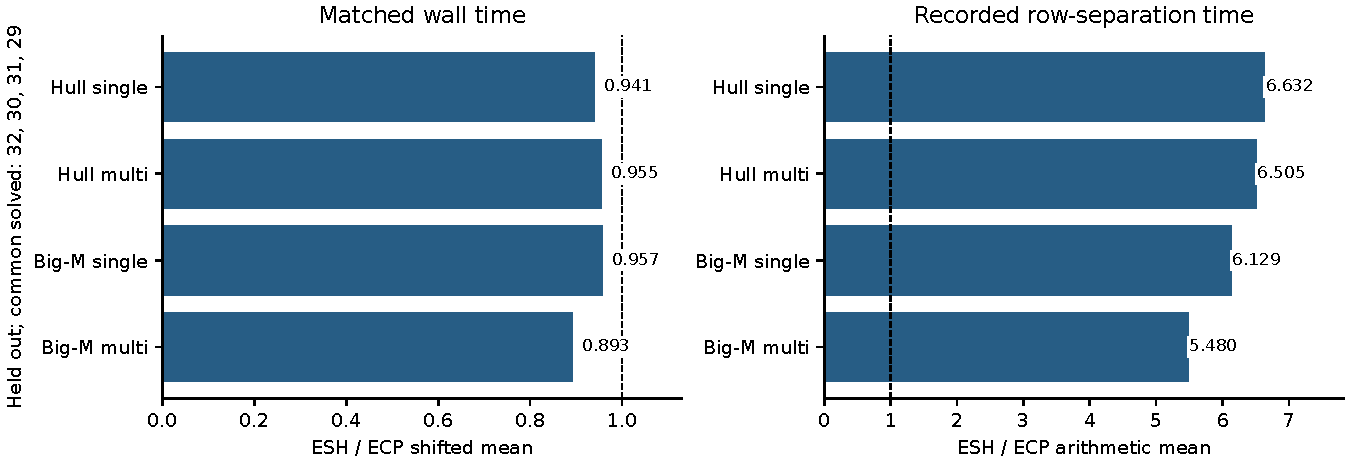
\includegraphics[width=\linewidth]{figures/cost_tradeoff.pdf}
\caption{The measured tradeoff on the same primary held-out cohorts. Left: ratio of shifted mean total wall time. Right: ratio of arithmetic mean recorded row-separation time per run. The two panels deliberately use different statistics and scales; neither is a per-cut comparison.}\label{fig:tradeoff}
\end{figure}

The means do not describe uniform or typical-case search savings. Hull-single median nodes are 9 for ESH versus 8 for ECP, median reduced NLP counts 4.5 versus 4, and median master times 0.336 versus 0.290 seconds. Hull-multi median nodes likewise reverse (14.5 versus 13.5), with median NLP counts tied at two. Cut and LP-iteration medians favor ESH in all four pairs; \cref{tab:work-medians} gives all paired medians. The mean node/NLP reductions concentrate in harder cases, and the aggregate telemetry alone does not establish a causal explanation.

Interior NLP counts coincide within each pair, with mean counts 19.41, 17.97, 18.97 and 17.45 in the table's order; their mean times lie between about 0.86 and 0.94 seconds. ECP shares this initialization cost by design. Single-tree master time includes callback NLP and cut work, so component times must not be summed. GDP root-search function counts were not recorded; the separate diagnostic counts in \cref{sec:oracle-empirical} cannot be imputed to these runs.

All 33 held-out ESH hull LP phases end with the recorded reason \texttt{stalled}; ECP hull has 30 stalled and three \texttt{no\_separating\_cuts} exits, identically for both tree modes. Maximum final perspective residuals are approximately $1.20\cdot10^{-5}$ for ESH and $6.21\cdot10^{-6}$ for ECP. Each big-M configuration has 32 stalled LP phases and one iteration-limit exit; a perspective-residual certificate is inapplicable to that formulation. These LP exits establish neither hull feasibility nor equality with an exact cone relaxation.

\subsection{Conic alternatives and numerical references}\label{sec:conic-results}
The exact quadratic mixed-integer hull solves all nine quadratic controls. Its all-nine shifted mean wall time is 0.455 seconds, compared with 2.280 for ESH hull single and 2.272 for ECP hull single; all prototype configurations solve these same nine cases. The held-out six-case means are 0.449, 2.282 and 2.283 seconds, respectively. \Cref{tab:quadratic} reports every configuration. The supplied exact conic formulation is approximately five times faster than hull single here. This is a useful negative control: favorable comparisons with generic formulations in \cref{tab:primary} do not extend to the best supported conic alternative tested. No general superiority over quadratic GDPs is inferred.

For the separate continuous-cone comparison, 40 of the 42 supported roots have optimal status. The remaining two have inaccurate optimal status. Define
\[
 \Delta=\frac{B_{\rm cone}-B_{\rm LP}}{\max\{1,|f_{\rm cone}|\}},
\]
where $B_{\rm cone}$ is the numerical cone dual estimate, $f_{\rm cone}$ its primal objective, and $B_{\rm LP}$ the initial hull LP bound. All 40 optimal-status differences are positive. Their medians are $1.10\cdot10^{-6}$ (ESH) and $1.07\cdot10^{-6}$ (ECP); 39 of 40 have magnitude at most $10^{-4}$ for each separator. The maxima, $1.32\cdot10^{-4}$ and $2.78\cdot10^{-4}$, both occur on the pilot large logsumexp instance (\cref{tab:roots}). Single- and multiple-tree initial LP bounds coincide and are counted only once. The target is the same intersection of individual hulls, not a big-M relaxation. These floating-point comparisons support numerical consistency, without certifying the duals, proving hull equality or ranking all final LP bounds.

The two inaccurate-status roots remain separate: pilot medium log has primal/dual residuals $5.83\cdot10^{-10}$/$2.63\cdot10^{-9}$ and absolute cone gap $1.67\cdot10^{-7}$; pilot large reciprocal has $7.20\cdot10^{-11}$/$8.82\cdot10^{-10}$ and gap $1.92\cdot10^{-7}$. Their comparisons remain in the data but do not enter the 40-root precision summary. Even an optimal-status cone dual remains an uncertified numerical estimate.

Each of the 14 supported small instances has all 27 assignments enumerated. Of 378 solves, 174 report optimal with feasible witnesses and 204 report infeasible; none is unresolved. Fresh original-model checks accept all 174 witnesses. Every one of the 182 accepted primary outcomes on these 14 instances satisfies $|f-f_{\rm ref}|\le T(f_{\rm ref})$, where $f_{\rm ref}$ is the best enumeration witness objective and $T$ is defined in \eqref{eq:comparison-tolerance}; the largest discrepancy consumes about 1.32\% of that tolerance. This is support from a separate formulation and solver, not an exact infeasibility certificate for the remaining assignments or an exact optimum certificate.

\subsection{External scope and interface effects}\label{sec:external}
The 351 original external records contain 239 accepted solves, 38 feasible open/unusable gaps, four invalid witnesses, 61 errors, seven missing witnesses and two unsupported cone inputs. \Cref{tab:legacy} keeps all of them in the scheduled denominator. ESH and ECP have identical accepted counts in every matched external configuration. Excluding all six norm-objective stress cases by expression type gives common-solved ESH/ECP ratios of 1.015, 0.969, 1.010 and 0.969 for hull single, hull multi, big-M single and big-M multi, respectively (\cref{tab:legacy-pairs}). Small timing differences change direction with tree mode in this unrepeated experiment. The generated accepted-count advantage does not transfer to this external set.
\begin{table}[tb]
\centering\small
\caption{Original external accepted counts, stratified by expression scope. The conic adapter supports 25/27 inputs; two exponential batch models are unsupported, not failed supported solves. Norm-objective cases are stress tests for the smooth oracle.}\label{tab:legacy}
\begin{tabular}{lrrrr}
\toprule
Method & All /27 & No norm /21 & Norm /6 & Errors \\
\midrule
ESH hull single & 19 & 17 & 2 & 4 \\
ECP hull single & 19 & 17 & 2 & 4 \\
ESH hull multi & 20 & 18 & 2 & 4 \\
ECP hull multi & 20 & 18 & 2 & 4 \\
ESH big-M single & 20 & 18 & 2 & 4 \\
ECP big-M single & 20 & 18 & 2 & 4 \\
ESH big-M multi & 20 & 18 & 2 & 4 \\
ECP big-M multi & 20 & 18 & 2 & 4 \\
GDPopt LOA & 12 & 12 & 0 & 8 \\
SHOT big-M & 16 & 12 & 4 & 7 \\
Gurobi big-M & 12 & 12 & 0 & 7 \\
SCIP big-M & 19 & 13 & 6 & 7 \\
Exact conic hull & 22 & 17 & 5 & 0 \\
\bottomrule
\end{tabular}

\end{table}

Four norm cases, \texttt{CLay0204.l2}, \texttt{CLay0205.l2}, \texttt{CLay0304.l2} and \texttt{CLay0305.l2}, trigger nonfinite-gradient errors in all prototype configurations. The two successful norm cases remain in the same stress stratum. GDPopt has Ipopt failures on all six norm cases and subproblem-status errors on both batch models. These errors establish neither original-model infeasibility nor a general limitation of subgradient or conic methods.

All seven original farm inputs cause writer division-by-zero errors in each GAMS big-M interface (21 errors). All three GAMS methods also return incomplete batch-processing witnesses because the unused original variable \texttt{storageTankSize\_log[10]} is undefined. The full-witness gate rejects those three results. Consequently the original full-set timing penalties cannot be interpreted purely as solver-search performance.

The cone adapter solves 22 of its 25 supported inputs. Two farm cases retain open gaps, and \texttt{CLay0204.l2} has an invalid original linear-distance witness despite an optimal status. On the 19 models in both the no-norm and conic-supported strata, all eight prototype/conic timing comparisons share 17 common solved instances. The conic shifted mean is 0.928 seconds versus 2.225--3.255 seconds for the prototype configurations (ratios 0.285--0.417). This conditional timing advantage is not coverage dominance: the cone formulation leaves \texttt{FLay05} open, although several prototype configurations solve it, and \texttt{FLay06} remains open. Unsupported exponential cases and nonsmooth stress cases do not enter this supported-scope timing comparison.

\subsection{What the ablations establish}\label{sec:ablations}
Disabling integer-point NLP recovery reduces accepted outcomes from 69/72 to 1/72 on the four single-tree configurations and all 18 pilots (\cref{tab:ablations}). There are still 369 interior NLP solves per configuration across its 18 cases, so this is not an NLP-free algorithm. The 72 modified runs contain 62 stalled statuses, nine time limits and one accepted solution, ESH hull on the pilot small log instance. Of the stalled runs, 53 have no accepted incumbent and nine have a valid incumbent with an open gap; all nine time limits lack an accepted incumbent. No returned witness is invalid and no interface error occurs. Fast early stalls are unsuccessful outcomes, not runtime improvements.

These results identify integer-point NLP recovery as practically important to this prototype. They do not prove that convex GDP solution mathematically requires NLP subproblems, or contradict the conditional finite-separation results. Retained states do not include every rejected candidate and cut history, so all stalls cannot be attributed to one tolerance or numerical mechanism. This negative result defines the measured method as NLP-assisted.

Enabling fractional user cuts leaves accepted counts unchanged. It does submit cuts: 1763 and 1487 for ESH/ECP hull, and 16435 and 17864 for ESH/ECP big-M, across their respective 18 pilots. Cuts occur on 17/18 ESH-hull instances and all instances for the other configurations. Common-solved user-cuts/default timing ratios are 1.000, 1.006, 1.006 and 1.016. These small differences provide no persuasive benefit in the unrepeated pilot comparison. They concern the fixed node threshold $0.05$, not the proposed residual-calibrated rule.

\subsection{Outcome-triggered baseline follow-ups}\label{sec:followups}
Two separately declared follow-ups diagnose the original failures without replacing them. Tightening only Gurobi's \texttt{FeasibilityTol} to $10^{-8}$ on all nine trigonometric controls gives nine valid original-model witnesses instead of three, and six accepted solves instead of three. All medium cases now close the gap; all large cases remain valid but open at the solver limit. Per-instance times change in both directions (\cref{tab:trig-followup}); this is not a general speedup claim.

The legacy follow-up changes only initial values on the seven farms and batch processing, for each GAMS solver: widths start at their existing positive affine lower bounds, and the unused trailing batch variable at its existing bound. Algebra, bounds, options and checking tolerances remain fixed. All 24 calls then return; 23 witnesses are valid and 11 are accepted (\cref{tab:initialization}). Gurobi contributes four solves, SCIP seven and SHOT zero. Gurobi's remaining invalid witness is \texttt{FLay05}, with a nonoverlap-row residual about $7.94\cdot10^{-6}$ against $1.1\cdot10^{-6}$.

Missing interface information still matters: the initialized batch Gurobi log reports objective 679365.3263389, bound 679307.9309222 and gap 0.0084\%, but GAMS exports \texttt{OBJEST=NA}. The unchanged gate therefore records an unusable gap. This is missing exported information despite a native closed-gap report, not evidence that Gurobi failed to close its gap. No log value is substituted after the fact. SHOT's normal termination on several farms likewise does not establish a closed gap; native logs retain its default nonconvex classification and loose bounds. These follow-ups qualify the original baseline rankings while leaving the matched ESH/ECP comparison unchanged.

\section{Discussion}\label{sec:discussion}
The controlled comparison answers a practical implementation question. Once a GDP solver already maintains term-specific interiors, recovers integer-point incumbents with NLPs, and supports the same master formulations, replacing point tangents by radial cuts can reduce enough outer work to repay the extra function evaluations. The measured benefit is modest: the single-tree conditional timing advantage remains about 4--6\% across three schedules. The larger formulation and tree effects suggest that separator choice should be assessed within the complete solver architecture. Aggregate means alone would overstate how consistently ESH reduces search, because several node and NLP medians favor ECP.

This finding is distinct from a new relaxation or algorithmic foundation. Perspective cuts, logic-based outer approximation, radial supporting points, and NLP-assisted single-tree methods have established precedents (\cref{sec:related}). The contribution here is the matched GDP experiment, the accompanying representation and oracle-cost diagnostics, and the explicit reconciliation of exact separation statements with the recorded numerical behavior. The residual-calibrated omission rule and counterexamples make that interpretation more precise. Their proofs are included to expose the assumptions needed to use the method, without a priority claim for elementary convexity or compactness arguments.

Several controls prevent a broader performance conclusion. An independently optimized ECP method could omit interior searches; the present comparison deliberately retains them, along with their effect on initial tangents. The generated controls share structures, parameter streams and size prefixes, and contain only a few seeds. The repeated runs change execution order but retain the search seed. Small aggregate differences therefore describe these matched schedules; they are not estimates over an independent population of applications. The preliminary cone pass also means that the held-out set was untuned rather than wholly unseen.

The external and conic results identify where the positive finding stops. Equal external accepted counts provide no evidence of wider ESH coverage. Missing interface values, original-model witness violations and initial-value export failures affect the external baseline rankings, as the separate follow-ups demonstrate. On supported quadratic and external comparisons, exact cone formulations can be substantially faster. The study does not include a general mixed-integer conic OA solver, so its results cannot rank the prototype against that broader approach. Nonquadratic functions also need not be nonconic; the exponential, logarithmic and reciprocal controls have explicit supplied cone representations.

The recovery ablation is especially informative. The tested implementation derives much of its practical success from solving selected continuous subproblems. Finite fixed-residual separation does not ensure that its finite-tolerance callbacks will produce usable incumbents or close a gap within a time limit. The retained logs establish the observed stalls and open gaps, but do not contain complete candidate and cut histories that would identify a single cause for every failure. Similarly, enabling the tested fractional user cuts adds work without improving accepted counts. These outcomes delimit the present implementation; they do not invalidate separation-based convex optimization or the residual-calibrated rule, which was not implemented in the frozen study.

Finally, validity and numerical certification are different obligations. The exact proofs require in-domain evaluations, compact candidate sets, and enforcement of old cuts. The implementation retains full tangent offsets and validates recovered incumbents, but it does not provide interval-certified coefficients, certified cone duals, or a certified normalization domain near zero selection weights. Original-model checks and independent arithmetic/reference comparisons strengthen the empirical evidence while remaining numerical checks. The manuscript and supplement keep this boundary explicit so that the reported solves, theoretical statements and software behavior refer to the same precisely scoped study.

\section{Conclusion}\label{sec:conclusion}
In the matched NLP-assisted GDP implementation studied here, radial separation gives a small but repeatable computational benefit over point tangents. It generates fewer cuts on average but spends substantially more recorded row-separation time per run. The advantage depends on the formulation, tree policy, shared initialization and tested instances, and it does not carry over to higher external accepted counts. Supported exact conic alternatives have lower common-solved mean times in these comparisons, while external coverage is mixed.

The mathematical analysis states what holds independently of these timings: valid perspective inequalities, finite fixed-residual separation under explicit compactness and enforcement conditions, and a safe residual-calibrated treatment of small weights. The diagnostic and counterexamples show that these guarantees imply neither universal cut dominance nor a general linear objective-error bound without additional joint regularity. With the complete model specifications, retained negative outcomes, original-model validation and reproducible artifacts, the study gives a concrete basis for deciding whether radial separation is worth its cost in a particular GDP solver.

\bibliographystyle{plainnat}
\bibliography{references}
\appendix
\section{What separation guarantees}\label{sec:theory}
This appendix states what can and cannot be inferred from successful separation. The results assume exact arithmetic and retained valid cuts unless stated otherwise. They support the comparison and do not form a new general convergence framework; their compactness arguments give no useful polynomial runtime bounds.

\subsection{Uniform margins for the two policies}
For one row $g$ on its compact convex box $C_r$, write
\[
 D_r=\operatorname{diam}(C_r),\quad R_r=\max_{x\in C_r}\|x\|_2,
 \quad F_r=\max_{x\in C_r}|g(x)|,\quad
 \|\nabla g(x)\|_2\le L_r\quad(x\in C_r).
\]
For a term row, $C_r=C$; for a global row, $C_r=C\times[0,1]^m$. Enlarged boxes include any bounded epigraph. Indices are suppressed when treating one row. A zero-diameter domain or a row with $L=0$ is checked directly. In the latter case the row is constant on the domain and a positive value eliminates its term, or proves global infeasibility.

\begin{lemma}[Separation and normal bounds]\label{lem:margin}
Let $g(p)=v>0$, $p\in C_r$, $L,D>0$. The ECP tangent violates its inequality at $p$ by $v$. Suppose also that a fixed anchor $\bar x\in C_r$ satisfies $g(\bar x)\le-\delta$ for $\delta>0$. Let $z=\bar x+s(p-\bar x)$, $0<s<1$, satisfy $g(z)=0$. Then the ESH tangent satisfies
\begin{equation}\label{eq:margin}
 \ell_z(p)\ge\frac{\delta v}{LD}.
\end{equation}
Every tangent normal has $\|a_z\|_2\le L$, and every perspective-cut normal has
\begin{equation}\label{eq:normal-bound}
 \|(a_z,b_z)\|_2\le K:=\sqrt{L^2+(F+LR)^2}.
\end{equation}
\end{lemma}
\begin{proof}
For ECP, $\ell_p(p)=g(p)=v$. Existence of $s\in(0,1)$ follows by continuity from the negative anchor value and positive exterior value. The supporting inequality at $\bar x$ yields
\[
 -\delta\ge g(\bar x)\ge a_z^T(\bar x-z)=-s a_z^T(p-\bar x),
\]
so $a_z^T(p-\bar x)\ge\delta/s$. The gradient bound, integrated along the segment, gives
$v=g(p)-g(z)\le L\|p-z\|_2\le LD(1-s)$. Consequently
\[
 \ell_z(p)=a_z^T(p-z)=(1-s)a_z^T(p-\bar x)
 \ge(1-s)\delta/s\ge\delta v/(LD).
\]
Finally, $|b_z|\le|g(z)|+\|a_z\|_2\|z\|_2\le F+LR$, proving \eqref{eq:normal-bound}.
\end{proof}
The anchor may differ by row; a shared anchor is an implementation convenience. Its actual row value, not an auxiliary NLP termination code, must establish the strict margin. ECP supplies a fallback when such an anchor is unavailable, without any Slater assumption. The proof also works for bounded chosen subgradients when the row is Lipschitz on the box: the supporting inequality at the anchor holds for every chosen subgradient, so a special directional-derivative-maximizing choice is unnecessary. This extension is not implemented.

\subsection{Integral candidates and objective bounds}
\begin{theorem}[Finite fixed-residual rejection]\label{thm:integral}
Fix $\eps>0$. Suppose master candidates satisfy all bounds, affine constraints, indicator logic, integrality, and previously retained cuts. Whenever a global or selected-term nonlinear row exceeds $\eps$, generate an ECP cut, or an ESH cut with a row-specific fixed positive anchor margin, for at least one such row. Retain every generated cut. Only finitely many such rejection iterations are possible. Thus an iteration process that keeps producing candidates either finds one with every relevant nonlinear row at most $\eps$ or exhausts its master candidates. This applies to both hull and valid finite-big-$M$ masters.
\end{theorem}
\begin{proof}
Assign each rejected candidate to a row for which a cut was generated. For a fixed nonconstant term row, restrict attention to the subsequence assigned to that row. Its term is active at all these candidates. If $p$ generated a cut and $q$ is a later candidate in this subsequence, the retained cut gives $\ell_z(q)\le0$, whereas \cref{lem:margin} gives $\ell_z(p)>\eps$ for ECP or $\ell_z(p)>\eps\delta/(LD)$ for ESH. Cauchy--Schwarz and $\|a_z\|_2\le L$ imply respectively
\[
 \|p-q\|_2>\eps/L\quad\hbox{or}\quad
 \|p-q\|_2>\eps\delta/(L^2D).
\]
When the term is selected, its hull copy equals $x$ and its big-$M$ deactivation vanishes, so this argument is valid in either master. A global row has the same argument in $(x,y)$ coordinates without an activity condition. Each compact box can be covered by finitely many balls whose diameters are smaller than the appropriate positive distance; at most one point of the subsequence lies in each ball. There are finitely many rows. Constant positive rows eliminate their term or the global master after one cut. Summing the finite rowwise bounds proves the assertion.
\end{proof}
The theorem does not require optimal master candidates, a globally solved NLP, or feasibility of inactive alternatives. It bounds nonlinear rejections, not all possible iterations of an algorithm trying to close an objective gap. In exact arithmetic, a valid outer approximation has optimum at most the GDP optimum. For an inexact master solve, the solver's valid minimization bound, rather than its incumbent objective, supplies the lower bound $B$. A residual-feasible point is not necessarily exactly feasible and does not automatically supply an upper bound on the exact problem. An independently validated exactly feasible point of objective $U$ together with $U-B\le\eta$ establishes feasible $\eta$-optimality; exact optimality requires zero gap. Fixed-residual separation alone guarantees neither an exact incumbent nor closure of this gap.

\subsection{Fractional residuals and small selection weights}
For each lifted term row define
\begin{equation}\label{eq:weighted-residual}
 r(\nu,\lambda)=
 \begin{cases}
 \lambda[g(\nu/\lambda)]_+,&\lambda>0,\\
 0,&(\nu,\lambda)=(0,0),
 \end{cases}\qquad [a]_+=\max\{a,0\}.
\end{equation}
This is continuous on the scaled bounded domain: $0\le r\le\lambda F$ controls its limit at zero weight. A small unscaled row residual and a small weighted perspective residual are different criteria.

\begin{theorem}[Residual-calibrated fractional separation]\label{thm:fractional}
Fix $\eps_p>0$ and a positive global-row tolerance. At every fractional hull candidate satisfying all previously retained cuts, separate at least one term row with $r>\eps_p$, or a global row exceeding its tolerance, using ECP or ESH as in \cref{lem:margin}. Retain all cuts. There are finitely many unsuccessful separation iterations before every residual meets its tolerance or no relaxation candidate exists.
\end{theorem}
\begin{proof}
For a term row with $r>\eps_p$, its ECP transformed violation is exactly $\lambda g(p)=r>\eps_p$. Its ESH transformed violation is at least $r\delta/(LD)>\eps_p\delta/(LD)$. The coefficient norm is bounded independently of $\lambda$ by \eqref{eq:normal-bound}. Thus a later block satisfying that cut is separated from its generating block in $(\nu,\lambda)$ by more than $\eps_p/K$ or $\eps_p\delta/(LDK)$. These blocks range over a compact scaled box. Apply the finite-cover argument row by row, adding the global-row argument in \cref{thm:integral}. A positive constant term row gives $g\lambda\le0$ and needs at most one cut.
\end{proof}
Let $U_r\ge\max_{p\in C}[g_r(p)]_+$ be a valid finite row bound. It is safe to skip the row without computing $p$ whenever
\begin{equation}\label{eq:safe-skip}
 \lambda U_r\le\eps_p.
\end{equation}
Indeed $r\le\lambda U_r$; if $U_r=0$ the row is always satisfied, and otherwise every block requiring separation has $\lambda>\eps_p/U_r$. A conservative $U_r$ can follow from interval bounds or a gradient bound and a reference value. Tight bounds need not be cheap. This rule both justifies omission and places a positive lower bound on denominators that actually require evaluation.

The frozen implementation instead skips $\lambda\le\tau$ and tests $g_r(p)\le\eps$ on the remaining blocks. If that complete test succeeds, then
\begin{equation}\label{eq:fixed-cutoff}
 r_r\le\max\{\eps,\tau U_r\}.
\end{equation}
For checked blocks use $\lambda\le1$; for skipped ones use $\lambda\le\tau$. Consequently a fixed cutoff has no prescribed small absolute residual guarantee without $U_r$. At fixed $\tau>0$, cutting checked rows with unscaled violation above $\eps$ still gives a finite retained-cut packing argument, since their transformed margins exceed $\tau\eps$ for ECP, or $\tau\eps\delta/(LD)$ for ESH. This termination fact does not improve \eqref{eq:fixed-cutoff}. Row rescaling changes all these residuals, tolerances, and $U_r$.

The residual-calibrated policy \eqref{eq:safe-skip} is a theoretical alternative, not an implemented experimental setting. An intermediate LP objective remains a valid relaxation lower bound under exact valid cuts, but a stall or cap provides no completed residual test. In a fractional big-$M$ master the deactivation term may absorb a tangent's entire violation, so \cref{thm:fractional} is not a big-$M$ residual theorem.

\subsection{Geometric repair and the limit of an objective inference}
\begin{proposition}[Repair within one disjunction]\label{prop:repair}
Suppose each retained term is nonempty and has an anchor $\bar x_{ik}$ satisfying its box and affine rows and all its nonlinear rows with common margin $\delta_{ik}>0$. If $p_{ik}$ satisfies that term's box and affine rows, let $v_{ik}=\max_{j\in J_{ik}}[g_{ikj}(p_{ik})]_+$ (zero for an empty row set). Then
\begin{equation}\label{eq:repair}
 q_{ik}=\frac{\delta_{ik}p_{ik}+v_{ik}\bar x_{ik}}{\delta_{ik}+v_{ik}}\in S_{ik},
 \qquad \|q_{ik}-p_{ik}\|_2\le\frac{D v_{ik}}{\delta_{ik}+v_{ik}},
 \quad D=\operatorname{diam}(C).
\end{equation}
For a hull point whose checked blocks $\lambda_{ik}>\tau$ have $v_{ik}\le\eps$,
\begin{equation}\label{eq:hull-distance}
 \dist\left(x,\conv\bigcup_k S_{ik}\right)
 \le D\left(\sum_{k:\lambda_{ik}>\tau}\frac{\lambda_{ik}\eps}{\delta_{ik}+\eps}
       +\sum_{k:\lambda_{ik}\le\tau}\lambda_{ik}\right).
\end{equation}
If instead every row has weighted residual at most $\eps_p$, the distance is at most $D\sum_k\eps_p/\delta_{ik}$.
\end{proposition}
\begin{proof}
Convexity bounds each row at $q_{ik}$ by
$(\delta_{ik}v_{ik}-v_{ik}\delta_{ik})/(\delta_{ik}+v_{ik})=0$.
The box and affine rows are preserved by a convex combination. Also
$q_{ik}-p_{ik}=v_{ik}(\bar x_{ik}-p_{ik})/(\delta_{ik}+v_{ik})$, giving \eqref{eq:repair}. For every unchecked positive-weight term choose any feasible $q_{ik}$; its displacement is at most $D$. The convex combination $\sum_k\lambda_{ik}q_{ik}$ lies in the union hull, and the triangle inequality proves \eqref{eq:hull-distance}. Zero-weight terms contribute nothing and need no $p_{ik}$. Under the weighted-residual hypothesis, $\lambda_{ik}v_{ik}=\max_jr_{ikj}\le\eps_p$, and
$\lambda_{ik}v_{ik}/(\delta_{ik}+v_{ik})\le\eps_p/\delta_{ik}$.
Summing gives the final bound.
\end{proof}
These are distances to one disjunction's hull. Repairs for different disjunctions need not agree, nor satisfy the global constraints or coupled logic. Empty terms must be removed for this proposition or assigned zero weight; the earlier cut-validity results did not need this nonemptiness condition.

\begin{example}[No linear intersection error bound from term interiors]\label{ex:intersection}
On $0\le x,y\le1$, impose a single-term constraint $x^2-y\le0$, a global row $y\le0$, and minimize $-x$. The term has anchor $(0,1)$ and nonlinear margin one. The exact feasible point is $(0,0)$ and its objective is zero. For $0<\eps\le1$, the point $(\sqrt\eps,0)$ satisfies the global row exactly and the term with residual $\eps$, but its objective underestimation is $\sqrt\eps$. For every fixed $K>0$, $\sqrt\eps>K\eps$ when $0<\eps<1/K^2$. Thus separate-term Slater margins cannot imply a uniform $O(\eps)$ objective-error bound for their intersection with global constraints. Duplicating the alternative gives the same example with a two-term disjunction. A joint metric error bound or other joint regularity would be an additional assumption.
\end{example}

\begin{proposition}[Convergence in value without a rate]\label{prop:value}
Let a sequence of lifted candidates contained in one common compact domain satisfy the affine hull system and relaxed global logic. Suppose all global positive residuals and weighted perspective residuals tend to zero. If each candidate minimizes a valid outer relaxation of $\mathcal H$, its objective tends to the optimum $v_{\mathcal H}$. The conclusion also holds when candidate suboptimality tends to zero. If instead the candidates retain integral indicators and original integer coordinates and optimize valid outer relaxations of the GDP, the corresponding assertion holds for the GDP optimum.
\end{proposition}
\begin{proof}
Continuity of all residuals, including \eqref{eq:weighted-residual} at zero weight, makes every cluster point feasible for $\mathcal H$. Compactness supplies cluster points. Every relaxation optimum is at most $v_{\mathcal H}$; therefore candidate values are at most $v_{\mathcal H}+o(1)$. Every convergent candidate subsequence has limiting objective at least $v_{\mathcal H}$. If the full objective sequence did not converge to $v_{\mathcal H}$, a subsequence bounded away from it would, by compactness, contain a convergent subsequence contradicting these two bounds. In the integral case, replace $v_{\mathcal H}$ by the GDP optimum in the upper-bound argument. The bounded integer-coordinate set is closed, so every cluster point retains integrality and the lifted constraints enforce the original selected terms; its objective is therefore at least the GDP optimum. If the target feasible set is empty, no such compact sequence with vanishing residuals can exist.
\end{proof}
This is a limiting statement, not finite exact convergence or a convergence rate. A fixed residual or fixed positive weight cutoff alone does not provide its hypotheses.

\subsection{Single-tree execution requires an oracle contract}\label{sec:tree-contract}
\begin{theorem}[Conditional single-tree residual conclusion]\label{thm:single-tree}
Assume the compact-domain conditions above and the following exact-arithmetic solver contracts.
\begin{enumerate}
 \item The finite MILP master is solved completely in the absence of resource limits. Every old lazy cut is enforced for final feasibility. At callbacks violating an old cut, an existing cut is re-enforced without adding fresh cuts. Each such old-cut resolution episode finishes in finite time. Fresh nonlinear rejection iterations occur only at candidates satisfying all old cuts.
 \item Every potentially accepted integer candidate is tested against the original global and selected-term rows. A row above a fixed positive residual tolerance produces a valid rejecting cut with the uniform margin in \cref{lem:margin}. Inability to obtain such a cut is a failure, not acceptance.
 \item Any heuristic NLP point proposed as an exactly feasible incumbent is independently validated against bounds, affine and nonlinear rows, fixed values, integrality, logic, and the original objective. Failed NLP solves do not exclude an assignment without a separate valid infeasibility proof.
 \item Fractional cutting is disabled, capped at finitely many cuts, or obeys a retained-cut uniform-margin condition such as \cref{thm:fractional} or its fixed-positive-cutoff variant. Other optional refinement also contributes only finitely many cuts.
\end{enumerate}
Then only finitely many distinct nonlinear integer rejection iterations and permitted fractional cut iterations occur. Under the complete-master-solver contract, the algorithm eventually establishes master infeasibility or produces an integer point meeting the nonlinear residual tolerance. An exactly feasible incumbent $U$ and a valid master bound $B$ additionally establish feasible $\eta$-optimality whenever $U-B\le\eta$.
\end{theorem}
\begin{proof}
Contract~1 places fresh integer rejection candidates under \cref{thm:integral}; their number is finite. Contract~4 bounds fractional and other refinement. Old-cut repetitions finish in finite time by contract~1. After finitely many additions, the complete finite MILP solve either has no feasible candidate or processes an integer candidate that cannot be rejected above the prescribed residual tolerance. Contract~2 supplies the residual conclusion. Under exact cut validity, master infeasibility proves GDP infeasibility. Contracts~1 and~3 supply valid $B$ and $U$ for the stated objective inequality. That inequality, rather than final master status alone, establishes the objective conclusion.
\end{proof}
These are substantive conditions on solver behavior, not consequences of choosing a callback API. A solver may present a callback candidate violating an earlier lazy cut; generating additional cuts at that point does not by itself justify packing it as a new separated point. Unlimited repeated user cuts, especially after solver purging, are likewise outside the proof. The frozen numerical implementation is not asserted to satisfy this exact termination contract. Feasibility within numerical tolerance must retain that qualification even if the numerical master gap closes.

\subsection{Approximate roots and finite arithmetic}\label{sec:arithmetic}
An exact tangent at an approximate boundary point remains valid provided its full constant $g(z)-\nabla g(z)^Tz$ is retained. It need not pass through $z$. Deleting $g(z)$ can invalidate the cut: for $g(x)=x^2-1$ and $z=1/2$, the artificial boundary tangent becomes $x\le1/2$ and excludes feasible $x=1$. The true tangent is $x\le5/4$ and remains valid. Validity alone does not establish useful separation. A robust oracle should check the transformed cut's actual violation, fall back to ECP if needed, and report failure if neither cut reliably rejects the candidate.

\begin{proposition}[A sufficient certified arithmetic scheme]\label{prop:arithmetic}
On a compact candidate domain, let the exact valid cut be $q^Tw\le d$. Suppose computed coefficients satisfy the certified bound
\[
 |(\widetilde q^Tw-\widetilde d)-(q^Tw-d)|\le E
 \quad\hbox{for every domain point }w.
\]
Then $\widetilde q^Tw\le\widetilde d+E$ is valid. If the exact generating violation is at least $\kappa$, its violation of this relaxed computed cut is at least $\kappa-2E$. If later candidates can violate stored cuts by at most $\rho$, uniform bounds $\kappa>2E+\rho$ and $\|\widetilde q\|_2\le\widetilde K$ with $\widetilde K>0$ give a minimum separation distance $(\kappa-2E-\rho)/\widetilde K$.
\end{proposition}
\begin{proof}
At every point satisfying the exact cut, the computed left-minus-right expression is at most $E$, proving validity after relaxation. At its generating point, that expression is at least $\kappa-E$, hence at least $\kappa-2E$ after relaxation. At a later accepted point it is at most $\rho$. Subtract the two inequalities and apply Cauchy--Schwarz to obtain the distance bound. The same finite-cover arguments then apply.
\end{proof}
For example, certified coefficient errors $|\widetilde q_j-q_j|\le e_j$ and $|\widetilde d-d|\le e_d$, with $|w_j|\le W_j$, give $E=e_d+\sum_j e_jW_j$. Nonlinear evaluation errors also need bounds before a residual test becomes certified. Ordinary double-precision gradients, NLP statuses and MILP bounds do not supply these enclosures. The numerical study instead reports explicitly defined residual and gap tests.

\section{Representation and cut-geometry diagnostics}\label{sec:oracle}
A point tangent depends on the algebraic representation of a feasible set. A radial boundary construction has a restricted invariance when its anchor is held fixed. The relationship between ESH and cutting planes for gauge reformulations is already established \citep{serrano2020}; the results here isolate consequences that can be checked by the actual separator without a full GDP solve.

\subsection{Equivalent rows and fixed-anchor invariance}
\begin{proposition}[Boundary halfspace invariance]\label{prop:invariance}
Let $g$ be convex and differentiable on a neighborhood of its box, and let $\phi$ be convex, differentiable and strictly increasing on an interval containing the values of $g$, with $\phi(0)=0$ and $\phi'(0)>0$. The row $\widehat g=\phi\circ g\le0$ defines the same feasible set and is convex. For a fixed strict anchor and exterior point, exact rowwise ESH gives the same halfspace for $g$ and $\widehat g$, including after the hull transform. At an exterior point $p$ with $v=g(p)>0$ and $\phi'(v)>0$, the ECP inequality for $\widehat g$ is
\begin{equation}\label{eq:reexpressed-ecp}
 \nabla g(p)^T(x-p)\le-\frac{\phi(v)}{\phi'(v)},
\end{equation}
instead of the right side $-v$ for $g$.
\end{proposition}
\begin{proof}
Strict monotonicity and $\phi(0)=0$ preserve the signs of all row values. Convexity of $g$, monotonicity of $\phi$ and convexity of $\phi$, in that order, prove convexity of the composition. The common segment has the same boundary point $z$ for both rows. At it, $\nabla\widehat g(z)=\phi'(0)\nabla g(z)$ and both row values vanish. The affine coefficients, including the homogeneous perspective coefficients, are therefore multiplied by the same positive factor. At $p$, the chain rule gives tangent
$\phi(v)+\phi'(v)\nabla g(p)^T(x-p)\le0$; division by $\phi'(v)>0$ proves \eqref{eq:reexpressed-ecp}.
\end{proof}
A positive linear $\phi$ preserves point tangents too, but a general convex increasing transformation does not. Convexity implies $\phi(v)\le v\phi'(v)$ for $v>0$, so under this transformation the ECP inequality at the \emph{same} exterior point is no stronger than the original one. This does not compare subsequent master trajectories or runtime. The proposition requires the same anchor: the auxiliary interior optimization itself can respond to a changed representation. It also requires exact boundary roots. Approximate root tolerances, row scaling and finite arithmetic need not preserve the halfspace.

\subsection{A scalar recurrence and its interpretation}
\begin{proposition}[An arbitrarily long point-tangent transient]\label{prop:scalar}
For $a\ge2$, consider
\begin{equation}\label{eq:scalar}
 \min\{-x:0\le x\le2,\quad g_a(x)=\exp(a(x-1))-1\le0\}.
\end{equation}
Every instance has feasible interval $[0,1]$, optimum $-1$, and strict anchor zero. Starting from the box alone, or the box plus a tangent at zero, the first master optimum is $p_0=2$. One exact ESH cut gives $x\le1$. With exact ECP and all cuts retained, successive master optima satisfy
\begin{equation}\label{eq:scalar-recurrence}
 p_{k+1}=p_k-\frac{1-\exp[-a(p_k-1)]}{a},\qquad p_k>1.
\end{equation}
For any fixed $0<\eta<1$, reaching $p_k\le1+\eta$ requires $k>a(1-\eta)$ cuts. Nevertheless $p_k\downarrow1$.
\end{proposition}
\begin{proof}
The anchor tangent gives $x\le(e^a-1)/a$, whose right side exceeds two for $a\ge2$: $e^2>5$, and the derivative of $e^a-1-2a$ is positive for $a\ge2$. It thus leaves the box optimum unchanged. The segment from zero to any $p>1$ meets the unique boundary at $z=1$, where $g_a'(1)=a>0$; ESH gives $a(x-1)\le0$. The ECP tangent at $p_k$ yields
\[
 x\le p_k-\frac{g_a(p_k)}{g_a'(p_k)}
 =p_k-\frac{1-\exp[-a(p_k-1)]}{a}.
\]
For $u>0$, $0<1-e^{-u}<u$. Therefore this new bound is strictly between one and $p_k$, and all older upper bounds are weaker. This proves the recurrence for the actual master optima, rather than merely for a proposed iteration. Each decrease is strictly less than $1/a$, so $2-p_k<k/a$. If $p_k\le1+\eta$, then $1-\eta\le2-p_k<k/a$, proving the lower bound. Monotonicity and the lower bound one give a limit $p_*\ge1$; if $p_*>1$, continuity in the recurrence gives a strictly positive limiting decrement, a contradiction.
\end{proof}
Equation~\eqref{eq:scalar-recurrence} is precisely Newton's method for the equation $g_a(x)=0$, started from the exterior point. The example exhibits a representation-dependent initial transient, not a failure of asymptotic Newton convergence: with $e_k=p_k-1\to0$, Taylor expansion gives
\[
 e_{k+1}=\tfrac{a}{2}e_k^2+O(e_k^3)\quad\text{for fixed }a.
\]
This elementary mechanism is not GDP-specific. Nor is the iteration lower bound a runtime lower bound: ESH spends additional row evaluations on its boundary search. Large $a$ creates conditioning and overflow concerns in finite arithmetic. A transformed function-residual tolerance is not a common geometric accuracy criterion across $a$; a numerical diagnostic should instead use $\max\{0,p_k-1\}$, which is also the objective error here, and count evaluations.

\subsection{Centered geometry and explicit non-dominance}
For the centered ellipsoid row $q(x)=x^TQx-1$, $Q\succ0$, take anchor zero and $p=rQ^{-1/2}u$ with $r>1$ and $\|u\|_2=1$. The boundary is $z=Q^{-1/2}u$. ESH gives $z^TQx\le1$, whereas ECP gives
\[
 z^TQx\le\frac{r^2+1}{2r}=1+\frac{(r-1)^2}{2r}>1.
\]
Thus ESH dominates for this centered geometry. A convex increasing representation change as in \cref{prop:invariance} preserves the ESH halfspace and weakens or preserves the exterior-point tangent. This accounts for the selected centered diagnostic cases; it is not a general dominance statement.

\begin{example}[Neither policy generally dominates]\label{ex:nondominance}
Let $g(x_1,x_2)=x_1^2+x_2^2-1$ on $[-2,2]^2$, $p=(2,0)$ and $\bar x=(0,9/10)$. ECP gives $x_1\le5/4$. Solving the segment-circle intersection yields
\[
 z_1=\frac{162+20\sqrt{157}}{481},\qquad
 z_2=\frac9{10}-\frac9{20}z_1,
 \qquad z_1^2+z_2^2=1,
\]
and ESH gives $z_1x_1+z_2x_2\le1$. Direct bounds on the square root give $0.85<z_1<0.87$ and $0.50<z_2<0.52$. The point $(1.2,1)$ satisfies ECP, but its ESH left side exceeds $1.2(0.85)+0.50=1.52>1$. The point $(1.3,-2)$ violates ECP, but its ESH left side is less than $1.3(0.87)-2(0.50)=0.131<1$. Both witnesses belong to the common box. Consequently neither halfspace contains the other. They are witnesses about the outer approximations, not feasible disk points. Setting $\lambda=1$ transfers this non-dominance to the perspective cuts.
\end{example}
These examples explain why cut count, cut depth at one candidate and total solver benefit must be measured separately. They justify a controlled experiment without assuming which policy must win.

% Stage 3 owns the empirical diagnostic subsection below this marker.
% It must preserve the theory above and report frozen scalar/ellipsoid records,
% analytic oracle wrappers, evaluation counts, stopping criteria and scope.

\subsection{Evaluation of the frozen separator}\label{sec:oracle-empirical}
A solver-free experiment invokes the actual frozen \texttt{LBESH.\_esh\_cuts} routine with counted analytic value/gradient wrappers and the actual nonlinear-row container. It evaluates the cut algorithm, not the Pyomo/SymPy expression compiler. Exponential wrappers use \texttt{expm1} for stable evaluation. The anchor is prescribed, no GDP or optimization subproblem is solved, and every ESH call is checked to exclude ECP fallback. Both cut and feasibility tolerances are $10^{-12}$; bisection stops at a parameter-bracket width below $10^{-10}$.

For the scalar example, the initial master is the box alone for every representation, including $a=1$. The base row $x-1$ is also passed through the separator; a real model extractor would instead recognize it as affine. After each cut its floating-point coefficients update the scalar upper bound by direct division. All cases stop at the common geometric criterion $(x-1)_+\le10^{-8}$, rather than a representation-dependent function residual. \Cref{tab:oracle,fig:oracle-cost} show the complete design. ECP uses 1, 5, 6, 8, 12, 20 and 36 cuts for the base row and $a=1,2,4,8,16,32$; ESH uses one throughout. Each ECP cut requires two value calls and one gradient; each ESH cut requires 37 values and one gradient, including 34 bisection evaluations and one value each at the candidate, anchor and tangent point. Bisection does not stop early at an exact zero. Thus ESH uses more total value calls through $a=8$, despite using fewer cuts. Scalar ESH bounds equal one at recorded precision; ECP's largest terminal geometric error is $2.56\cdot10^{-11}$ and recurrence disagreement is at most $2.23\cdot10^{-16}$.
\begin{figure}[tb]
\centering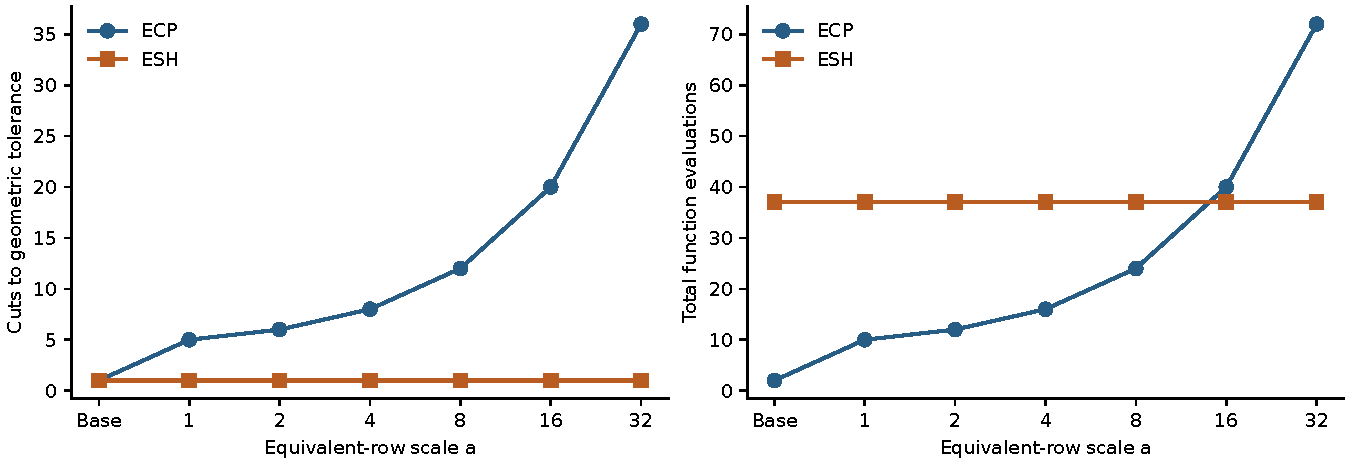
\includegraphics[width=\linewidth]{figures/oracle_cost.pdf}
\caption{Scalar representation diagnostic using the frozen separator. Fewer cuts do not imply fewer function evaluations. The design fixes the anchor and uses the same geometric stopping tolerance for every equivalent row.}\label{fig:oracle-cost}
\end{figure}

The two-dimensional design uses $Q=I$ or $\operatorname{diag}(1,4)$, anchor zero, and $p=rQ^{-1/2}(\cos\theta,\sin\theta)$ with $r\in\{1.25,1.75\}$ and $\theta=2\pi k/16$, $k=0,\ldots,15$. Both policies are tested on the base row $q(x)=x^TQx-1$ and the six transformed rows $\exp(aq(x))-1$ with $a\in\{1,2,4,8,16,32\}$, giving $2\cdot2\cdot16\cdot7\cdot2=896$ individual cuts. Every point lies in $[-2,2]^2$. After unit-normal scaling, ESH support constants differ from the analytic supporting constants by at most $4.45\cdot10^{-16}$; normal errors are below $10^{-12}$. ECP constants differ from their own analytic ECP constants by less than $10^{-9}$; these constants generally differ from the ellipsoid's supporting constants. Each cut $n^Tx+c\le0$ passes the analytic ellipsoid support check $\sqrt{n^TQ^{-1}n}+c\le10^{-10}$. These floating-point comparisons do not constitute interval certificates.

At the disk point $(1.75,0)$, ESH depth is 0.75 for every representation; ECP depth falls from 0.589286 for the base row to 0.008929 for $a=32$. This invariance is numerical evidence for this fixed centered geometry, where the two normals are parallel. The off-center control from the preceding subsection yields ESH depth 0.715590 versus ECP's 0.75, and reproduces both non-containment witnesses. It prevents the centered examples from suggesting uniform cut dominance.

Nine timing samples are retained for every scalar sequence and two-dimensional cut. Scalar median times range approximately 41--85 microseconds for ESH and 10--533 microseconds for ECP across representations. They exclude imports and creation of the counted function and oracle objects, but include oracle calls, per-call row/container construction and Python bookkeeping. At these durations, concurrent work and measurement overhead preclude a robust speed interpretation. There are no MILP, NLP or anchor-computation costs here. The diagnostic establishes a representation-sensitive mechanism and its oracle cost; it does not show that this mechanism explains every GDP outcome.

\section{Controlled models and reference formulations}\label{app:models}
This appendix specifies the tested models independently of their implementation. Indices are $i=0,\ldots,n-1$, $p\in\{0,1\}$ and $j\in\{0,1,2\}$; neighbor indices are taken modulo $n$. Let $y_{ij}$ be exclusive mode indicators, $\sum_jy_{ij}=1$. Each family/size/seed has identifier \texttt{lbesh.FAMILY.SIZE.sSEED}. Sizes and seeds are specified in \cref{sec:design}.

\subsection{Technology allocation}
Let $U_i>0$, $D_i=1.1U_i$, weights $w_{ip}>0$, cross coefficient $c_i>0$, mode fixed charges $F_{ij}\ge0$, operating coefficients $a_{ij}\ge0$, capacity fractions $\kappa_{ij}$ and resource coefficients $h_{ip}>0$. For $j=1,2$, define
\begin{equation}\label{eq:generator-cost}
 C_{ij}(x_i)=U_i a_{ij}\left[\sum_{p=0}^1w_{ip}\phi(x_{ip}/D_i)
 +c_i\phi\!\left((x_{i0}+x_{i1})/(2D_i)\right)\right].
\end{equation}
The five function laws and second derivatives are
\begin{center}\small
\begin{tabular}{lll}\toprule
Family & $\phi(z)$ & $\phi''(z)$\\\midrule
exp & $(e^{3z}-1)/(e^{1.5}-1)$ & $9e^{3z}/(e^{1.5}-1)$\\
log & $-\log(1-z)/\log 2$ & $1/((1-z)^2\log 2)$\\
reciprocal & $(1-z)^{-1}-1$ & $2/(1-z)^3$\\
quadratic & $4z^2$ & $8$\\
trig & $(1-\cos(1.5z))/(1-\cos(0.75))$ & $2.25\cos(1.5z)/(1-\cos(0.75))$\\\bottomrule
\end{tabular}\end{center}
Every law has $\phi(0)=0$ and $\phi(1/2)=1$; normalization does not equalize curvature. Variables satisfy $0\le x_{ip}\le U_i$ and $0\le t_i\le T_i$, where
\[
 T_i=1.05\max_{j=1,2} C_{ij}(U_i,U_i).
\]
The off mode imposes $x_{i0}+x_{i1}\le0$ and $t_i=0$; operating mode $j$ imposes $x_{i0}+x_{i1}\le U_i\kappa_{ij}$ and $C_{ij}(x_i)\le t_i$. The objective is
\[
 \min\ \sum_i t_i+\sum_{i,j}U_iF_{ij}y_{ij}.
\]
Define the explicit production witness $\bar x_{i0}=0.28U_i$, $\bar x_{i1}=0.22U_i$. The global rows are
\begin{align*}
 x_{i0}+x_{i1}&\le U_i &&(i=0,\ldots,n-1),\\
 \sum_i x_{ip}&\ge\sum_i\bar x_{ip} &&(p=0,1),\\
 \sum_{i,p}h_{ip}x_{ip}&\le1.08\sum_{i,p}h_{ip}\bar x_{ip},\\
 \sum_i\left(\frac{x_{i0}+0.35x_{i+1,1}}{U_i}\right)^2
 &\le1.08\sum_i\left(\frac{\bar x_{i0}+0.35\bar x_{i+1,1}}{U_i}\right)^2.
\end{align*}
There are $n+4$ global rows, $6n$ disjunct rows, one nonlinear global row and $2n$ nonlinear disjunct rows.

For each seed a local Python \texttt{random.Random(seed)} stream generates unit data sequentially in the following order; each listed coordinate is a separate uniform draw:
\begin{center}\small
\begin{tabular}{ll}\toprule
Parameter (draw order) & Interval or fixed value\\\midrule
$U_i$ & $[0.8,1.2]$\\
$w_{i0},w_{i1}$ & $[0.75,1.25]$\\
$c_i$ & $[0.2,0.5]$\\
$(F_{i0},F_{i1},F_{i2})$ & $(0,\ [0.08,0.12],\ [0.25,0.35])$\\
$(a_{i0},a_{i1},a_{i2})$ & $(0,\ [1.05,1.25],\ [0.65,0.85])$\\
$(\kappa_{i0},\kappa_{i1},\kappa_{i2})$ & $(0,\ [0.58,0.68],\ 1)$\\
$h_{i0},h_{i1}$ & $[0.7,1.3]$\\\bottomrule
\end{tabular}\end{center}
No draw is rejected. Standard operation has a smaller fixed charge and larger operating coefficient than efficient operation for every unit. Standard is cheaper at zero production, while efficient operation admits production beyond the standard capacity. Thus neither alternative can eliminate the other by those comparisons alone.

The entire individual-variable box, even before enforcing global capacity, puts all three arguments in \eqref{eq:generator-cost} in $[0,10/11]$. The log/reciprocal singularity is therefore separated by at least $1/11$. For trig, $0\le1.5z\le15/11<\pi/2$, so both the first derivative and the displayed second derivative are nonnegative, and the latter is strictly positive. All laws are nondecreasing on this interval, and convex and continuously differentiable on an open neighborhood of it. Positive affine compositions and sums preserve convexity; subtracting $t_i$ preserves it. Congestion is a sum of affine squares. Monotonicity proves that $T_i$ accommodates the minimum epigraph cost everywhere in the box. This bound restricts redundant large epigraph values but excludes no optimal production decision.

Choose mode 1 everywhere, set $x=\bar x$ and $t_i=C_{i1}(\bar x_i)$. Standard capacity exceeds $0.50U_i$, product demands hold at equality, both resource budgets have 8\% slack, and the cost/box rows hold. This proves feasibility for every allowed draw independently of a solver. Finite variable bounds, continuity and the finite disjunctions imply a compact feasible set and attained finite optimum. The witness is a primal bound, not a known optimum.

\subsection{Coupled exponential regions}
Let centers $c_{ijp}$, positive scales $\alpha_{ijp}$, radii $R_{ij}$, coordinate prices $b_{ip}$ and fixed charges $F_{ij}$ be given. Each mode imposes
\begin{equation}\label{eq:generator-region}
 \sum_{p=0}^1\sum_{s\in\{-1,1\}}
 e^{s\alpha_{ijp}(x_{ip}-c_{ijp})}\le R_{ij}.
\end{equation}
The variables obey $-2\le x_{ip}\le2$, $0\le t\le9n$; the objective is
\[
 \min\ \sum_{i,p}b_{ip}x_{ip}+0.1t+\sum_{i,j}F_{ij}y_{ij}.
\]
Global rows impose $\sum_i x_{i0}\ge0$, $\sum_i x_{i1}\ge0.1n$ and
\[
 \sum_i(x_{i0}-0.5x_{i+1,1})^2\le t,\qquad
 \sum_{i,p}(x_{ip}-x_{i+1,p})^2\le0.55n.
\]
The generator again uses a fresh \texttt{random.Random(seed)} stream. For each unit it first draws two perturbations in $[-0.08,0.08]$ for each of the three centers $(-0.75,-0.35)$, $(0.25,0.70)$, $(0.80,-0.45)$, in that order. It then draws the six scales in $[1.7,2.3]$, three radii in $[4.8,5.6]$, prices $b_{i0}\in[0.8,1.2]$ and $b_{i1}\in[0.15,0.35]$, and three fixed charges in $[0.02,0.08]$. All draws are sequential uniform draws without rejection. There are four global rows (two nonlinear) and $3n$ nonlinear disjunct rows.

Each exponential has an affine argument; hence \eqref{eq:generator-region} is globally convex and smooth. Taking the logarithm of both sides gives an equivalent log-sum-exp sublevel set, although the implementation retains the sum-of-exponentials form. The other nonlinear rows are sums of affine squares. Each congestion difference is bounded in magnitude by three, proving the sufficient epigraph bound $9n$. Select mode 1 and set each point to its corresponding center. Region left sides then equal $4<4.8$; coordinates satisfy $x_{i0}\ge0.17$, $x_{i1}\ge0.62$, giving strict demand feasibility. Neighbor differences have magnitude at most 0.16, so variation is at most $2n(0.16)^2=0.0512n<0.55n$. Setting $t$ to the congestion value completes the witness. All rows are continuous on a finite box, proving boundedness and attainment as above. These invented positions and prices are geometry controls, not fitted facility-location data.

\subsection{Closed-cone representations}\label{app:cones}
The formulations here instantiate established conic perspective constructions \citep{ceria1999,bernal2024,gusev2026}; they are not a new reformulation theorem. Let
\[
 K_{\exp}=\operatorname{cl}\{(a,b,c):b>0,\ b e^{a/b}\le c\}.
\]
Its zero-scale slice is $b=0$, $a\le0$, $c\ge0$ \citep{cvxpycones}. We also use
\begin{equation}\label{eq:product-soc}
 ab\ge c^2,\ a,b\ge0
 \quad\Longleftrightarrow\quad
 \|(2c,a-b)\|_2\le a+b.
\end{equation}
Squaring the latter nonnegative sides yields $4c^2+(a-b)^2\le(a+b)^2$ and hence the equivalence.

For a weight $y\ge0$, copied normalized argument $z$ and auxiliary epigraph $q\ge0$, the four supported allocation laws have the following perspective epigraphs:
\begin{center}\small
\begin{tabular}{ll}\toprule
Law & Constraint\\\midrule
exp & $(3z,y,(e^{1.5}-1)q+y)\in K_{\exp}$\\
log & $(-\log(2)q,y,y-z)\in K_{\exp}$\\
reciprocal & $(q+y)(y-z)\ge y^2$, with both factors nonnegative\\
quadratic & $qy\ge4z^2$, with $q,y\ge0$\\\bottomrule
\end{tabular}\end{center}
For $y>0$, division gives $q\ge y\phi(z/y)$ in every case; for reciprocal, for example, $(q/y+1)(1-z/y)\ge1$. Copied box bounds give $0\le z\le(10/11)y$, so $z=0$ at $y=0$ and positive-weight log/reciprocal inputs remain uniformly in their domains. Each auxiliary can be set to zero on an inactive branch. At zero weight some individual epigraph cones also allow positive $q$, but the copied aggregate cost row has zero right side and strictly positive coefficients, forcing all such auxiliaries to zero. Thus inactive branches project to the origin and impose no spurious restriction. Positive coefficients make separate epigraphs exact: they can meet a copied cost budget if and only if their minimal values do. Copies of both production coordinates and $t_i$ are made for every mode, including off; they sum to original variables and obey their original scaled boxes, capacity rows and off-mode $t$ equality.

For a region-mode weight $y$ and copied point $u$, use four cones
\[
 (s\alpha_{ijp}(u_p-c_{ijp}y),y,r_{ps})\in K_{\exp},
 \qquad \sum_{p,s}r_{ps}\le R_{ij}y,
 \qquad -2y\le u_p\le2y.
\]
For $y>0$ these recover the perspective of \eqref{eq:generator-region}; at $y=0$, copied coordinates vanish and nonnegative $r_{ps}$ sum to at most zero, so all vanish. Global quadratic rows use \eqref{eq:product-soc} with one fixed nonnegative factor. Consequently continuous weights describe the intersection of each disjunction's exact bounded convex hull and the global rows, and integral weights recover the original model. This is not generally the full GDP hull. For fixed-assignment references, only the selected $y=1$ modes are retained; their analytic fixed-charge constant is added to primal and dual objectives. The translator reads generator coefficients, uses none of the prototype's expression extraction/cuts, and supplies no trig translation.

The independent mixed-integer quadratic adapter instead reads model expression trees. For
\[
 q(x)=x^TQx+a^Tx+c\le0,\qquad Q\succeq0,
\]
it introduces copies $\nu$, weight $\lambda$ and slack $s$ with
\begin{equation}\label{eq:quadratic-cone}
 \nu^TQ\nu\le s\lambda,\qquad
 s=-a^T\nu-c\lambda,\qquad s\ge0,\quad\lambda\ge0.
\end{equation}
Positive weights recover $\lambda q(\nu/\lambda)\le0$; zero weight forces $\nu=s=0$ through finite scaled bounds and the slack equality. Factoring $Q=A^TA$ gives a rotated second-order cone, recognized by Gurobi \citep{gurobi}. Explicit nonnegative affine-square sums are preserved: for $\sum_kw_k(A_kx+b_k)^2+a^Tx+c$, use $z_k=A_k\nu+b_k\lambda$ and $\sum_kw_kz_k^2\le s\lambda$. This avoids introducing apparent indefiniteness by expanding rank-deficient squares. Other expanded quadratic matrices undergo a conservative exact-rational PSD check on the represented binary floating-point coefficients, without eigenvalue clipping or regularization. ``Exact'' describes the formulation, not floating-point coefficients, witnesses or solver certificates.

The adapter also handles global nonnegative weighted norm sums through SOC epigraphs, and $a/d(x)$ with $a>0$ and nonnegative affine denominator through $a\le td$, $t,d\ge0$. The product forces $d>0$, preserving the domain even with a zero declared lower bound. A zero numerator requires a strictly positive declared denominator bound. These epigraphs are used only in convex monotone positions. Global exponential expressions, nonconvex quadratics, nonlinear equalities lacking supported convex orientations, missing copied-variable bounds, OR/nested/reused disjuncts, disjunct objectives, SOS and nonfixed GDP indicators inside disjunct rows are rejected. Each disjunction copies all variables occurring in any of its alternatives into every alternative; global-only variables need not be copied. Logical constraints use Pyomo's logical-to-linear transform. The closed perspectives contain no epsilon parameter.

\subsection{External-model scope}\label{app:legacy-scope}
The tested inputs are the archived local builders, not a claim of bitwise identity with a published formulation. Their source files and parameter data are fingerprinted. GDPlib and Pyomo distribute the model families \citep{gdplib,pyomoexamples}; source docstrings trace batch processing to Ravemark and LOGMIP, positioning to Duran--Grossmann and Gavish--Horsky--Srikanth, small batch to Kocis--Grossmann, circles to Lee--Grossmann, layouts to Sawaya, and the basic-step example to Papageorgiou--Trespalacios. Modified circles, alternate farms and the $\ell_2$ layout objective are explicitly model variants.

A structural audit of all 27 models orients every nonlinear inequality as convex on its effective domain. Quadratic rows have nonnegative diagonal quadratic terms, batch expressions are positive sums of affine exponentials, farm area constraints use positive constants divided by positive width, and the six norm objectives are positive sums of Euclidean norms. The latter are convex with bounded subgradients, but ordinary gradients are undefined at zero. They are not examples of unbounded norm gradients. All flat-XOR structure extractions succeed; this does not imply every smooth-oracle or compactness hypothesis holds.

\begin{center}\small
\begin{tabularx}{\linewidth}{lrlX}\toprule
Source family / identifiers & Count & Class & Qualification\\\midrule
GDPlib batch\_processing & 1 & C & Missing cycle-time upper bounds; automatic epigraph unbounded.\\
GDPlib positioning, small\_batch & 2 & B & Smooth bounded original coordinates; automatic epigraph unbounded.\\
Circles2D3, modified, Circles3D4 & 3 & B & Same epigraph qualification.\\
CLay0203/0204/0205/0303/0304/0305, l1 & 6 & C & Respectively 6/12/20/6/12/20 distance auxiliaries without upper bounds.\\
The same six CLay variants, l2 & 6 & C & Same auxiliaries, plus nonsmooth norm objective and unbounded epigraph.\\
FLay02/03/03\_alt\_1/03\_alt\_2/04/05/06 & 7 & A & Affine propagation gives compact boxes and positive widths.\\
basic\_step & 1 & A & Finite box, smooth quadratic rows, affine objective.\\
ex1\_Lee & 1 & B & Smooth bounded original coordinates; unbounded epigraph.\\\bottomrule
\end{tabularx}\end{center}
Class A denotes the analytic compact/smooth data of the extracted lift (eight models); B has compact smooth original coordinates but an unbounded automatic objective epigraph (six); C records further missing hypotheses (13). None certifies anchors, master behavior or termination. \Cref{sec:theory} explains how one may justify bounded epigraphs mathematically; the frozen implementation does not install those bounds.

Farm widths initially have declared lower bound zero, but affine rows imply positive minima (1, 1, 5, 1, 3, 1, 1 in the listed order), and affine enclosure rows imply finite bounds; extraction transfers these facts to the box. The original GAMS initialization failures concern the raw initial values, not a negative or zero width feasible under those affine rows. In batch processing, each positive term of a time-budget sum gives a finite cycle-time bound, but this tightening is absent from the frozen master box. Layout auxiliaries can be replaced by absolute coordinate differences without increasing their positive-weight objectives; coordinate-box-derived upper bounds therefore give an optimization-equivalent bounded formulation, but change the full feasible set and were not imposed here. Relaxed layouts can still place centers at coincident points, so feasible nonoverlap does not remove the nonsmooth-oracle issue.

The 21-model no-norm stratum excludes all six $\ell_2$ models; it does not assert all theorem assumptions. The cone adapter supports 25 models, excluding both exponential batch models, so its intersection with the no-norm stratum has 19. These sets are fixed by expressions and adapter scope, independently of solver outcomes. The compact data list every full identifier.

\section{Detailed computational comparisons}\label{app:computational}
The following tables supplement the main comparisons without changing their cohorts. The file \texttt{data/records.csv} supplies every individual benchmark outcome, objective, bound, wall time and retained work metric for all 1464 runs, including failures. Full witness checks and native outputs are in the research bundle. \texttt{data/table\_values.json} supplies the exact displayed table entries. Table values are regenerated from immutable records, not transcribed from narrative results.

\begin{table}[htbp]\centering\small
\caption{Every primary accepted-status discrepancy between ESH and ECP. ESH solves; ECP retains a feasible open gap.}\label{tab:discordant}
\begin{tabular}{llrrr}
\toprule
Instance suffix & Split & Pair & ESH (s) & ECP (s) \\
\midrule
log.large.s130363 & held out & Hull single & 65.18 & 120.87 \\
logsumexp.large.s104729 & pilot & Hull single & 101.46 & 120.83 \\
log.large.s130363 & held out & Big-M single & 113.67 & 120.79 \\
log.large.s155921 & held out & Big-M single & 56.44 & 120.83 \\
log.large.s104729 & pilot & Big-M multi & 107.00 & 120.80 \\
\bottomrule
\end{tabular}

\end{table}
\begin{table}[htbp]\centering\small
\caption{Three schedules, unchanged solver seed: accepted counts (out of 33) and full-cohort PAR10 seconds for each repetition.}\label{tab:repeat-outcomes}
\begin{tabular}{lrr}
\toprule
Method & Solved: runs 1/2/3 & PAR10: runs 1/2/3 \\
\midrule
ESH hull single & 33/33/33 & 6.061/5.924/5.834 \\
ECP hull single & 32/32/32 & 50.791/50.628/50.630 \\
ESH big-M single & 33/33/33 & 11.164/10.868/10.649 \\
ECP big-M single & 31/31/31 & 97.723/97.543/97.530 \\
\bottomrule
\end{tabular}

\end{table}
\begin{table}[htbp]\centering\small
\caption{Fixed common-solved cohorts across three repetitions: ESH/ECP shifted means in seconds, followed by their ratio.}\label{tab:repetitions}
\begin{tabular}{lrrr}
\toprule
Pair; fixed common & Run 1: ESH/ECP; ratio & Run 2 & Run 3 \\
\midrule
Hull single; 32 & 3.040 / 3.233; 0.941 & 2.983 / 3.138; 0.951 & 2.911 / 3.095; 0.941 \\
Big-M single; 31 & 4.294 / 4.484; 0.957 & 4.141 / 4.377; 0.946 & 4.107 / 4.380; 0.938 \\
\bottomrule
\end{tabular}

\end{table}
\begin{table}[htbp]\centering\small
\caption{Held-out ESH/ECP shifted wall-time ratios and common-solved counts in parentheses. Family scheduled counts are six except logsumexp (three); size scheduled counts are 11 each.}\label{tab:family-size}
\begin{tabular}{lrrrr}
\toprule
Stratum & Hull single & Hull multi & Big-M single & Big-M multi \\
\midrule
exp & 0.994 (6) & 0.944 (6) & 0.975 (6) & 0.871 (6) \\
log & 0.883 (5) & 0.950 (4) & 0.972 (4) & 0.872 (4) \\
logsumexp & 0.781 (3) & 0.857 (2) & 0.930 (3) & 0.864 (2) \\
quadratic & 1.000 (6) & 0.989 (6) & 0.990 (6) & 1.003 (6) \\
reciprocal & 0.922 (6) & 0.937 (6) & 0.894 (6) & 0.866 (5) \\
trig & 1.016 (6) & 0.998 (6) & 0.982 (6) & 0.860 (6) \\
small & 0.969 (11) & 0.959 (11) & 1.014 (11) & 0.987 (11) \\
medium & 0.984 (11) & 0.952 (11) & 1.002 (11) & 0.889 (11) \\
large & 0.877 (10) & 0.951 (8) & 0.865 (9) & 0.789 (7) \\
\bottomrule
\end{tabular}

\end{table}
\begin{table}[htbp]\centering\small
\caption{Formulation and tree contrasts on matched held-out common-solved cohorts. Ratios are of shifted wall-time means, with common counts in parentheses; cohort membership differs by contrast.}\label{tab:structure}
\begin{tabular}{lrr}
\toprule
Contrast & ESH ratio (common) & ECP ratio (common) \\
\midrule
Hull / big-M, single & 0.648 (33) & 0.652 (31) \\
Hull / big-M, multi & 0.508 (29) & 0.468 (29) \\
Single / multi, hull & 0.893 (30) & 0.866 (30) \\
Single / multi, big-M & 0.736 (29) & 0.676 (29) \\
\bottomrule
\end{tabular}

\end{table}
\begin{table}[htbp]\centering\scriptsize
\caption{Paired medians, ESH / ECP, on the same common-solved cohorts as \cref{tab:work}. Node/NLP mean savings do not uniformly persist at the median.}\label{tab:work-medians}
\begin{tabular}{lrrrrr}
\toprule
Pair & Cuts & LP iter. & NLP solves & Nodes & Master time (s) \\
\midrule
Hull single & 488.0 / 545.0 & 33.5 / 35.0 & 4.5 / 4.0 & 9.0 / 8.0 & 0.336 / 0.290 \\
Hull multi & 343.5 / 361.0 & 33.0 / 35.0 & 2.0 / 2.0 & 14.5 / 13.5 & 0.084 / 0.081 \\
Big-M single & 711.0 / 801.0 & 33.0 / 46.0 & 21.0 / 21.0 & 229.0 / 241.0 & 1.449 / 1.319 \\
Big-M multi & 462.0 / 591.0 & 30.0 / 45.0 & 9.0 / 9.0 & 757.0 / 840.0 & 0.930 / 1.363 \\
\bottomrule
\end{tabular}

\end{table}
\begin{table}[htbp]\centering\small
\caption{Exact quadratic hull context: shifted wall-time means in seconds on complete common cohorts. All listed methods solve all nine quadratic controls.}\label{tab:quadratic}
\begin{tabular}{lrr}
\toprule
Method & Held out (6) & All quadratic (9) \\
\midrule
Exact conic hull & 0.449 & 0.455 \\
ESH hull single & 2.282 & 2.280 \\
ECP hull single & 2.283 & 2.272 \\
ESH hull multi & 2.166 & 2.157 \\
ECP hull multi & 2.191 & 2.173 \\
ESH big-M single & 3.830 & 3.692 \\
ECP big-M single & 3.868 & 3.828 \\
ESH big-M multi & 4.240 & 4.285 \\
ECP big-M multi & 4.225 & 4.275 \\
\bottomrule
\end{tabular}

\end{table}
\begin{table}[htbp]\centering\small
\caption{External common-solved timing after excluding all norm-objective models by expression scope. Shifted means are seconds; ratios are ESH/ECP.}\label{tab:legacy-pairs}
\begin{tabular}{lrrrr}
\toprule
Pair & Common /21 & ESH (s) & ECP (s) & Ratio \\
\midrule
Hull single & 17 & 2.575 & 2.537 & 1.015 \\
Hull multi & 18 & 3.139 & 3.238 & 0.969 \\
Big-M single & 18 & 2.976 & 2.946 & 1.010 \\
Big-M multi & 18 & 2.267 & 2.341 & 0.969 \\
\bottomrule
\end{tabular}

\end{table}
\begin{table}[htbp]\centering\scriptsize
\caption{Pilot ablations. The first three numeric columns give accepted solves out of 18. Time ratio is user-cuts/default on their common-solved cases (18, 17, 17, 17); cuts and cases refer to all 18 user-cut runs. ``No int. NLP'' still includes interior NLP initialization.}\label{tab:ablations}
\begin{tabular}{lrrrrrr}
\toprule
Method & Default & No int. NLP & User cuts & Time ratio & Cuts & Cases \\
\midrule
ESH hull & 18 & 1 & 18 & 1.000 & 1763 & 17 \\
ECP hull & 17 & 0 & 17 & 1.006 & 1487 & 18 \\
ESH big-M & 17 & 0 & 17 & 1.006 & 16435 & 18 \\
ECP big-M & 17 & 0 & 17 & 1.016 & 17864 & 18 \\
\bottomrule
\end{tabular}

\end{table}
\begin{table}[htbp]\centering\small
\caption{Same-hull root diagnostic $\Delta$ on 40 optimal-status cone references. Two inaccurate references remain separate. The numerical differences are not certified errors.}\label{tab:roots}
\begin{tabular}{lrrrr}
\toprule
Separator & Minimum & Median & Maximum & $|\Delta|\le10^{-4}$ /40 \\
\midrule
ESH & 1.43e-07 & 1.10e-06 & 1.32e-04 & 39 \\
ECP & 4.69e-08 & 1.07e-06 & 2.78e-04 & 39 \\
\bottomrule
\end{tabular}

\end{table}
\begin{table}[htbp]\centering\small
\caption{All nine original/tightened Gurobi trigonometric pairs. S: accepted numerical solve; I: invalid witness; F: feasible open gap. The follow-up sets only \texttt{FeasibilityTol}$=10^{-8}$.}\label{tab:trig-followup}
\begin{tabular}{lrrrr}
\toprule
Size.seed & Original & Tightened & Original (s) & Tightened (s) \\
\midrule
small.s104729 & S & S & 1.267 & 1.724 \\
small.s130363 & S & S & 26.833 & 1.267 \\
small.s155921 & S & S & 1.318 & 1.670 \\
medium.s104729 & I & S & 5.677 & 4.980 \\
medium.s130363 & I & S & 10.843 & 14.960 \\
medium.s155921 & I & S & 8.338 & 3.775 \\
large.s104729 & I & F & 121.556 & 121.345 \\
large.s130363 & I & F & 121.532 & 121.297 \\
large.s155921 & I & F & 121.435 & 121.871 \\
\bottomrule
\end{tabular}

\end{table}
\begin{table}[htbp]\centering\small
\caption{Legacy initial-value follow-up. The corresponding originals contain seven writer errors and one invalid incomplete witness per solver. ``Open/missing gap'' retains valid witnesses whose exported bounds do not close the declared gap.}\label{tab:initialization}
\begin{tabular}{lrrrrr}
\toprule
Method & Runs & Valid & Solved & Open/missing gap & Invalid \\
\midrule
Gurobi big-M & 8 & 7 & 4 & 3 & 1 \\
SCIP big-M & 8 & 8 & 7 & 1 & 0 \\
SHOT big-M & 8 & 8 & 0 & 8 & 0 \\
\bottomrule
\end{tabular}

\end{table}
\begin{table}[htbp]\centering\small
\caption{Full scalar representation diagnostic. Value and gradient columns give total calls to the counted analytic wrappers; ESH's 37 values include 34 bisection evaluations.}\label{tab:oracle}
\begin{tabular}{lrrrrrr}
\toprule
Scale & ECP cuts & Values & Gradients & ESH cuts & Values & Gradients \\
\midrule
Base & 1 & 2 & 1 & 1 & 37 & 1 \\
1 & 5 & 10 & 5 & 1 & 37 & 1 \\
2 & 6 & 12 & 6 & 1 & 37 & 1 \\
4 & 8 & 16 & 8 & 1 & 37 & 1 \\
8 & 12 & 24 & 12 & 1 & 37 & 1 \\
16 & 20 & 40 & 20 & 1 & 37 & 1 \\
32 & 36 & 72 & 36 & 1 & 37 & 1 \\
\bottomrule
\end{tabular}

\end{table}
\clearpage


\section{Reproducibility and artifact provenance}\label{app:reproducibility}
\subsection{Delivered artifacts and numerical scope}
The accompanying source package contains the complete LaTeX manuscript, local bibliography, generated tables and figures, every individual benchmark outcome in compact JSON/CSV, all 51 generated parameter sets, and scripts that regenerate the displayed evidence. The separate frozen research supplement contains the solver and model sources, pinned environment declarations, saved schedules, raw witnesses and solver logs, conic references, analysis, and development provenance. It preserves third-party model licenses and source attributions. No solver binaries, environments or downloaded literature PDFs are redistributed. The manuscript and supplied figures build without access to the original repository, its literature directory, a network service or a solver license. The package has no claimed public archival identifier; it is supplied directly with the manuscript.

The file \texttt{README.md} gives executable instructions. The compact data description is \path{data/README.md}, its immutable-input hashes are in \path{data/provenance.json}, and its displayed entries are in \path{data/table_values.json}. The full supplement contains 9076 payload files and its embedded manifest (9077 archive members). Earlier pilots, failed exports, preliminary cone passes and superseded analyses remain as provenance; the final study uses \texttt{analysis\_v1} and the distinct eight benchmark batches identified in \cref{sec:design}. Repetitions and outcome-triggered follow-ups never replace primary outcomes.

Table regeneration redoes aggregation from the compact records, not primal validation. The separate independent audit re-evaluates witnesses in freshly constructed original GDPs, checks schedules and source metadata, and independently recomputes summary arithmetic. As stated in \cref{sec:acceptance}, it reuses the original-model checker. Acceptance uses \eqref{eq:accept-gap} and the criteria of \cref{sec:acceptance}, and cone-reference comparison uses \eqref{eq:comparison-tolerance}; these are numerical checks, not exact optimality, dual-feasibility or infeasibility certificates.

\subsection{Immutable identifiers and environments}
The following SHA-256 identifiers fix the research supplement, original executable-source freeze, and declared primary and supplementary schedules, respectively:
\begin{center}\scriptsize\ttfamily
f0399194ca1c9c57421965e236302c62e10eb72846ab807f936f18d9927d4b26\\
6c9eaf9898f04d08a12381879ab9bae79f83b800f0db9e4cc696ccbff6be84ad\\
1fd3118da6e10b5a47377ea00e3c8237262558b09764ba07ed5a66dc088090ca\\
6b45611e18668951d9794af8d7a80a8e9565a23323aee6d92cf1ad06cb4252a5
\end{center}
The primary and supplementary plan filenames are \path{study_plan_v1.json} and \path{supplementary_plan_v1.json}. Source-file and raw-record hashes, including both follow-up inputs and the post-freeze reference files, are recorded in the local provenance and full publication manifests. The publication archive is 38\,086\,636 bytes. It remains byte-identical to the completed research record; manuscript development did not alter the solver, instances or benchmark outcomes.

The benchmark software, processor, concurrency and effective solver options are specified in \cref{sec:settings}. The archived lockfiles reproduce the Python dependencies with \texttt{uv sync --frozen}; native GAMS, Gurobi and Ipopt installations and applicable licenses must be supplied separately for optimization reruns. The continuous CVXPY/Clarabel reference has its own lockfile under \texttt{lbesh\_research/conic\_reference\_env}. Historical environment declarations and native logs distinguish Gurobi 13.0.3 from GAMS/Gurobi 13.0.2. Hardware evidence comes from the saved logs, not an assumed identity with the machine used to typeset the paper. The writing environment used Python 3.13.11 and Matplotlib 3.11.2 for figure regeneration; the supplied generated files suffice for the TeX build.

\subsection{Reproduction commands and verification boundary}
From the extracted paper directory, the minimal build and local evidence checks are
\begin{verbatim}
latexmk -pdf -interaction=nonstopmode -halt-on-error main.tex
python scripts/regenerate.py
python scripts/check_evidence.py
\end{verbatim}
The generator requires Matplotlib for its two PDF figures; \texttt{--no-figures} regenerates tables and CSV using only the standard library. It verifies immutable input hashes and all 1464 unique batch--instance--method records before writing outputs. The evidence check also independently reconstructs all 51 parameter streams. The supplied source manifest and delivery checksums identify the exact manuscript version; \texttt{scripts/package.py} refreshes them after a correction.

The following verifies every research archive member against the manifest and extracts only regular, uniquely named files with safe relative paths into a new or empty directory:
\begin{verbatim}
python scripts/verify_supplement.py \
  supplement/publication_bundle_v1.tar.gz --extract research
python evidence/check_stage02.py --research-root research
\end{verbatim}
The second command checks the explicit analytic examples and selected frozen-source settings. Its research-root argument is mandatory, so relocation never silently bypasses source validation. From \texttt{research/code/minlp\_solver\_lab}, with the pinned Python environment active, the fresh full-study audit is
\begin{small}\begin{verbatim}
export PYTHONPATH="$PWD/instances/gdplib_src"
python lbesh_results_independent_audit.py \
  --fresh-validation \
  --compare-analysis results/lbesh_development/analysis_v1/analysis.json \
  --sensitivity results/lbesh_development/gurobi_trig_sensitivity_v1.jsonl \
  --legacy-initialization \
    results/lbesh_development/legacy_initialization_v1.jsonl \
  --out /tmp/lbesh-new-audit.json
\end{verbatim}\end{small}
The audit refuses an existing output file; choose a new path on each run. The explicit import path selects the extracted GDPlib sources even if a reused Python environment has an editable installation elsewhere. Set \texttt{OPENBLAS\_NUM\_THREADS}, \texttt{OMP\_NUM\_THREADS}, \texttt{MKL\_NUM\_THREADS} and \texttt{NUMEXPR\_NUM\_THREADS} to one. Optimization schedules and the separately pinned conic environment are documented in the archived \texttt{LBESH\_RESEARCH.md}; their declared commands and job orders are preserved in the plans. Executing those schedules is distinct from auditing their saved results.

As a portability check, both archives were relocated to a temporary directory, where a clean TeX build, regeneration of all 17 tables and two figures, the compact evidence check, the source/example check against the extracted research tree, and a fresh full-study audit all completed. The audit reconciled all 1464 benchmark outcomes and 6122 exported analysis fields, revalidated all 174 feasible enumeration witnesses, and found no cross-witness bound/status contradiction. Regenerated outputs matched the delivered files byte for byte. This check reused the existing pinned Python installation; it was neither a clean environment installation nor a rerun of optimization timings.

\end{document}
